% ============================================================
%  XJTU HOMEWORK TEMPLATE
%  Xi'an Jiaotong University — General Purpose Academic Report
% ============================================================
% ============================================================
%  DOCUMENT CLASS & CORE PACKAGES
% ============================================================
\documentclass[12pt]{article}
\usepackage{float}                  % [H] figure placement
\usepackage{graphicx}               % images and logo
\usepackage{geometry}               % page margins
\usepackage{fancyhdr}               % custom header/footer
\usepackage{xcolor}                 % colored text (red title)
\usepackage{setspace}               % line spacing control
\usepackage{titlesec}               % section heading style
\usepackage{parskip}                % space between paragraphs
\usepackage{amsmath}                % math environments
\usepackage{caption}                % caption formatting
\usepackage[T1]{fontenc}            % font encoding
\usepackage{mathptmx}               % Times New Roman (text + math)
\usepackage{hyperref}               % clickable links (optional)
% ============================================================
%  PAGE GEOMETRY — 1 inch margins on all sides
% ============================================================
\geometry{
    a4paper,
    top    = 1in,
    bottom = 1in,
    left   = 1in,
    right  = 1in,
    headheight = 1.6cm,
    headsep    = 0.5cm
}
% ============================================================
%  COLOR DEFINITIONS
% ============================================================
\definecolor{xjtu_red}{RGB}{175, 24, 28}     % XJTU brand red
\definecolor{header_gray}{RGB}{130, 130, 130} % subtle header text
\definecolor{rule_gray}{RGB}{200, 200, 200}   % decorative rules
% ============================================================
%  CAPTION STYLE — "Figure N: Description" format
% ============================================================
\captionsetup{
    labelfont  = {bf},
    textfont   = {small},
    labelsep   = colon,
    justification = centering,
    skip       = 6pt
}
% ============================================================
%  SECTION HEADING STYLE — 14pt, bold, XJTU red, underruled
% ============================================================
\titleformat{\section}
    {\fontsize{14}{17}\bfseries\color{xjtu_red}}
    {\thesection.}{0.6em}{}
    [\vspace{2pt}{\color{rule_gray}\titlerule[0.5pt]}]
\titlespacing*{\section}
    {0pt}{2ex plus 0.5ex minus 0.2ex}{1.2ex plus 0.2ex}
% ============================================================
%  LINE SPACING — body text
% ============================================================
\setstretch{1.15}
% ============================================================
%  GRAPHICSPATH — looks in current dir and screenshot/ subdir
% ============================================================
\graphicspath{{./}{./screenshot/}}
% ============================================================
%  HEADER SETUP
% ============================================================
\pagestyle{fancy}
\fancyhf{}  % clear defaults
\fancyhead[L]{%
    \fontsize{10}{12}\selectfont\color{header_gray}%
    Software Development\textbar{} Specialized Experiment 1%
}
\fancyhead[R]{%
    \includegraphics[height=1.0cm]{xjtu-logo-long.png}%
}
\fancyfoot[C]{\fontsize{10}{12}\selectfont\thepage}
\renewcommand{\headrulewidth}{0.5pt}
\renewcommand{\headrule}{%
    {\color{rule_gray}\hrule width\headwidth height\headrulewidth}%
}
\renewcommand{\footrulewidth}{0pt}
% ============================================================
%  DOCUMENT START
% ============================================================
\begin{document}
% ============================================================
%  COVER PAGE
% ============================================================
\begin{titlepage}
    \thispagestyle{empty}
    \centering
    \vspace*{1.2cm}
    \includegraphics[width=0.65\textwidth]{xjtu-logo-long.png}
    \vspace{1.0cm}

    {\color{xjtu_red}\rule{0.78\textwidth}{1.5pt}}
    \vspace{0.9cm}

    {\fontsize{22}{26}\bfseries\color{xjtu_red} Specialized Experiment 1}
    \vspace{0.55cm}

    {\fontsize{14}{18}\bfseries\color{xjtu_red}
        Short-term Rainfall Forecasting and Alert System
    }
    \vspace{0.9cm}

    {\color{xjtu_red}\rule{0.78\textwidth}{1.5pt}}
    \vspace{2.2cm}

    \begin{spacing}{2.0}
    {\fontsize{12}{16}\selectfont
        \begin{tabular}{r@{\hspace{0.8em}}l}
            \textbf{Class:}           & Software Development \\
            \textbf{Student Name:}    & Phanpasorn Laor-iam \\
            \textbf{Student Number:}  & 3125999087 \\
            \textbf{Faculty:}         & Electronic and Information Engineering \\
            \textbf{School:}          & Information and Communication Engineering \\
            \textbf{Teacher:}         & Professor Li Bo \\
            \textbf{Date:}            & \today \\
        \end{tabular}
    }
    \end{spacing}
    \vfill
    {\color{xjtu_red}\rule{0.78\textwidth}{1pt}}\\[0.5em]
    {\fontsize{10}{12}\selectfont\color{header_gray}%
        Xi'an Jiaotong University \quad\textbar\quad \the\year}
    \vspace{1.2cm}
\end{titlepage}

\pagestyle{fancy}
\setcounter{page}{1}

% ============================================================
\section{Introduction}
% ============================================================

The objective of this experiment is to construct a real-time rainfall monitoring system that utilizes external weather APIs and threshold-based logic to trigger alerts. The system is designed to support nowcasting (0--6 hours ahead), which is a critical component of modern urban flood management. By leveraging the OpenWeatherMap API and Streamlit, the project aims to automate rainfall detection and visualize rainfall intensity levels to enhance situational awareness during dynamic weather conditions.

The experiment is divided into three main components: API integration, Alert Logic Implementation, and Dashboard Development. The system development was structured into three primary technical phases using Python 3.10+ within the OpenCode Cloud environment.

First, in the API Integration phase, AI-assisted prompts were used to generate Python code utilizing the \texttt{requests} library to retrieve real-time weather data for specific locations, such as Bangkok, from the OpenWeatherMap API (\url{https://home.openweathermap.org/api\_keys}).

The implementation consists of three main Python scripts: \texttt{weather\_monitor.py}, \texttt{weather\_alert.py}, and \texttt{weather\_dashboard.py}, along with a \texttt{Prompt.md} file that documents all prompts used throughout the experiment.

% ============================================================
\section{API Integration}
% ============================================================

An API integration module was developed to retrieve real-time weather data from the OpenWeatherMap API. The system continuously monitors weather conditions for a specified city, including rainfall intensity, temperature, and timestamp information.

AI-generated code was used to implement the data acquisition process using the \texttt{requests} library. The system extracts key parameters such as rainfall amount, temperature, and date, which serve as inputs for subsequent alert logic and system analysis.

The prompt used to generate the implementation is shown in Fig.~\ref{fig:API_prompt}. The feedback and debugging process are illustrated in Fig.~\ref{fig:API_fb1} to Fig.~\ref{fig:API_fb3}, while the final output of the implementation is presented in Fig.~\ref{fig:API_output}.

\subsection{Initial Prompt}

\begin{figure}[H]
    \centering
    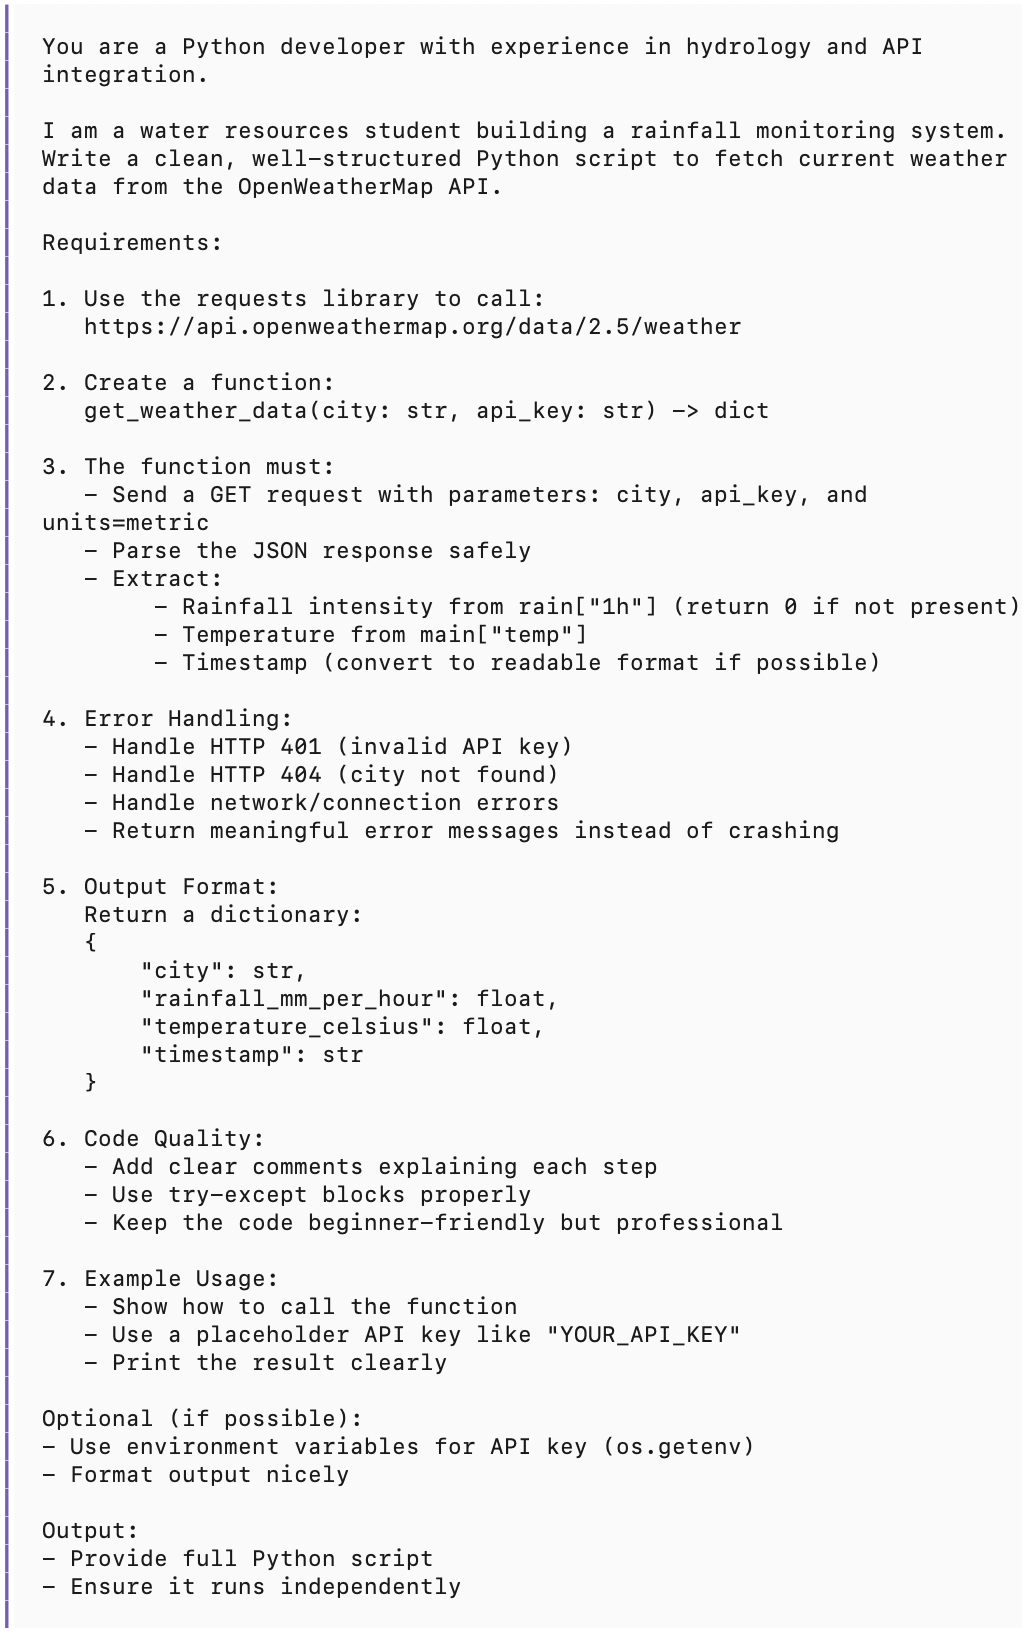
\includegraphics[width=0.9\textwidth]{experiment1-1st-prompt.png}
    \caption{Prompt for OpenWeatherMap API integration using the MiniMax agent}
    \label{fig:API_prompt}
\end{figure}

\subsection{Prompt Feedback}

\begin{figure}[H]
    \centering
    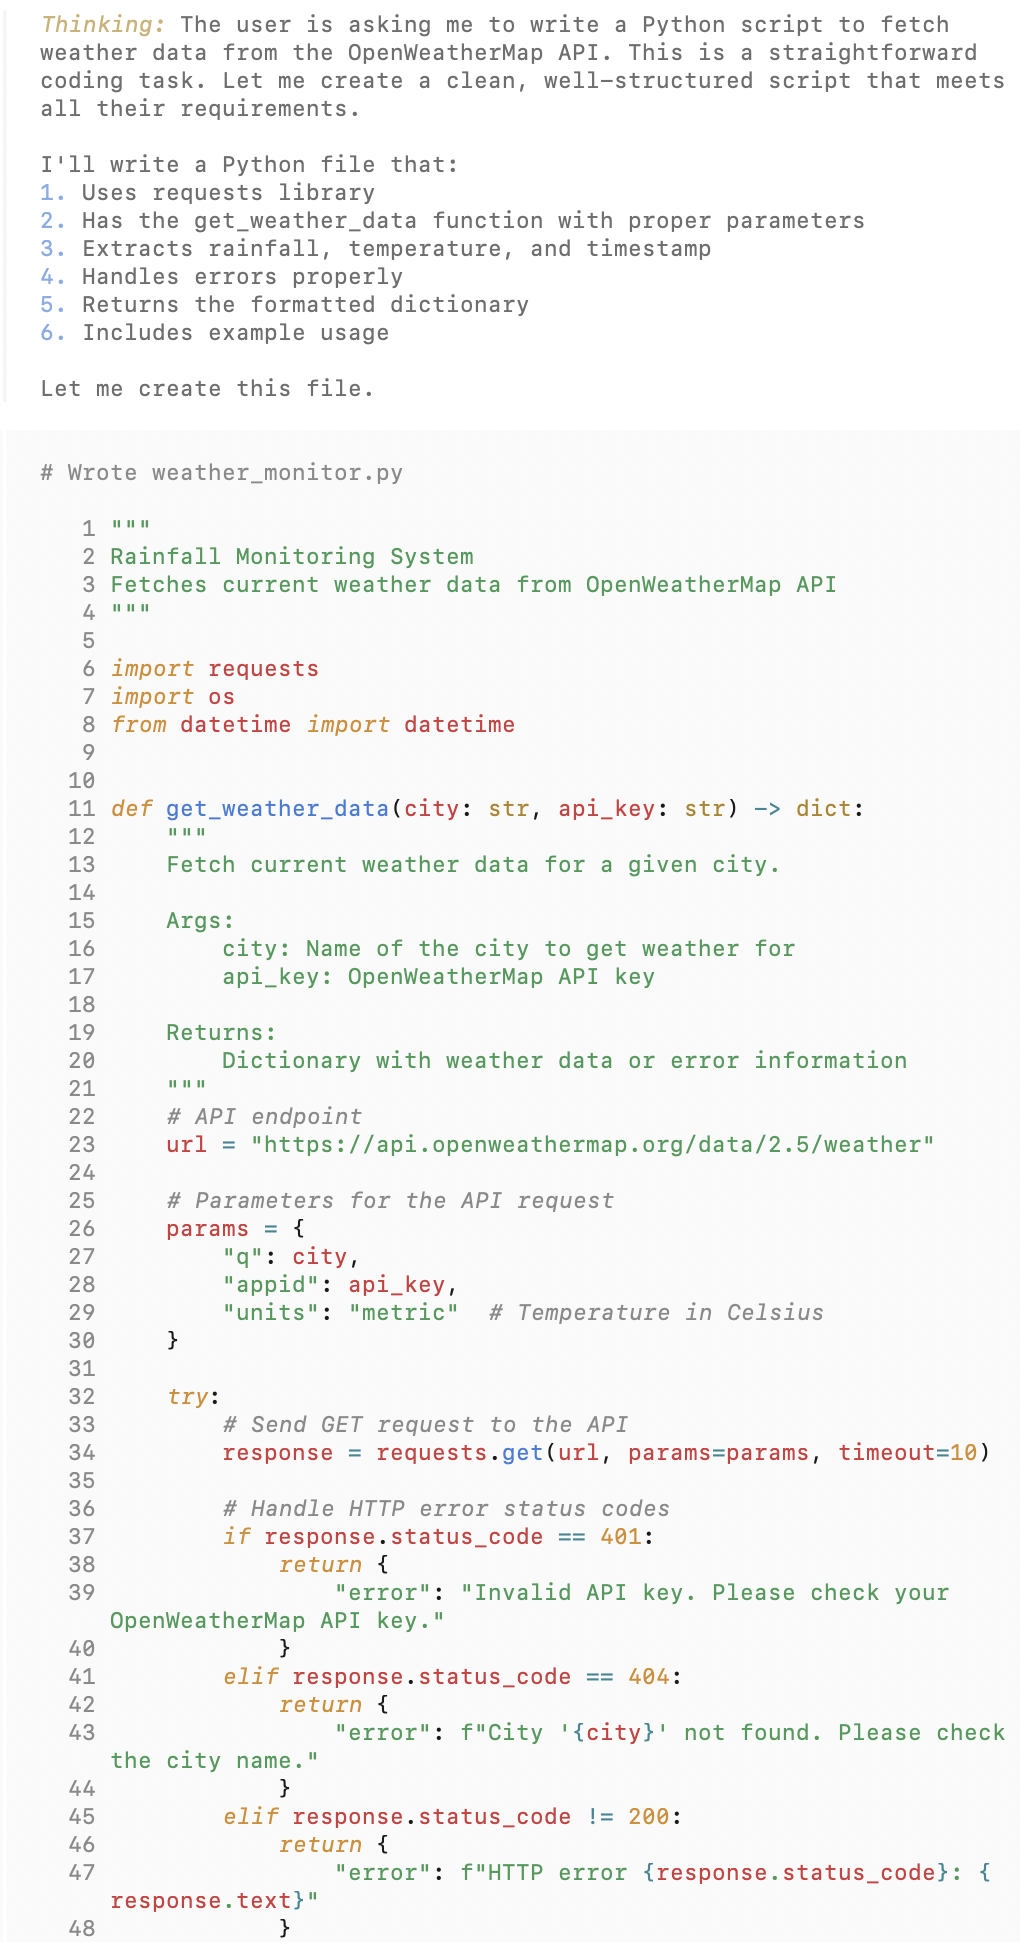
\includegraphics[width=0.9\textwidth]{experiment1-1st-prompt-feedback.png}
    \caption{Agent feedback after initial prompt submission}
    \label{fig:API_fb1}
\end{figure}

\begin{figure}[H]
    \centering
    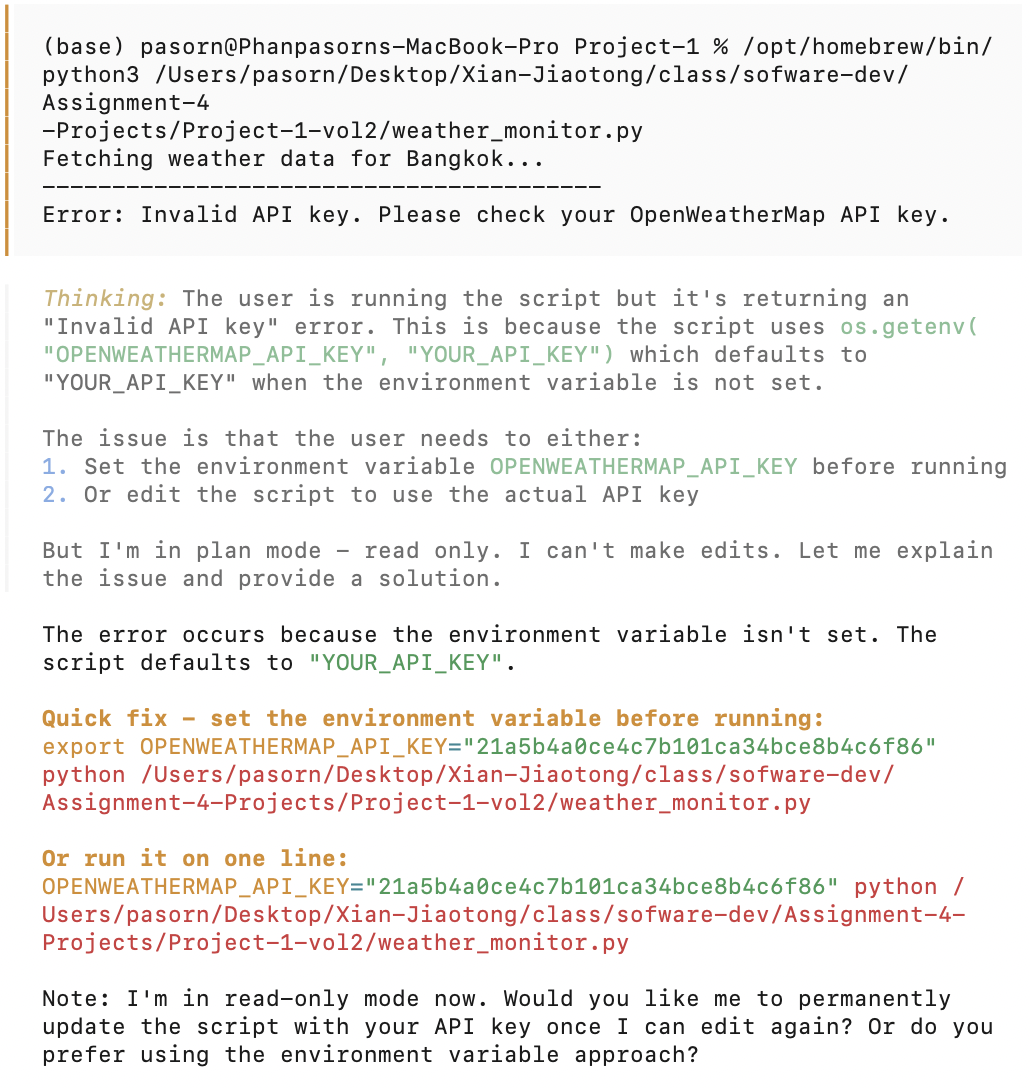
\includegraphics[width=0.9\textwidth]{experiment1-1st-prompt-error-fixed.png}
    \caption{Error identification and prompt refinement}
    \label{fig:API_fb2}
\end{figure}

\begin{figure}[H]
    \centering
    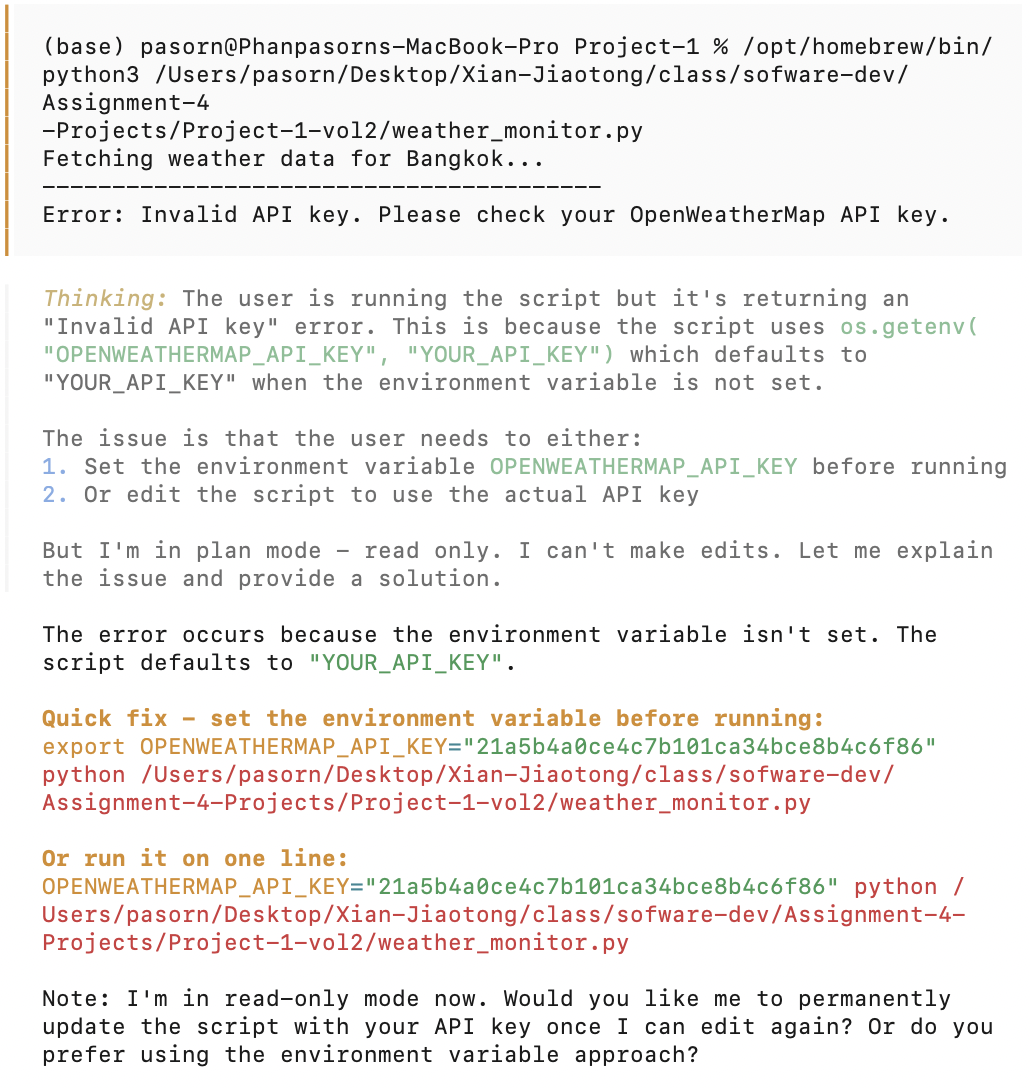
\includegraphics[width=0.9\textwidth]{experiment1-1st-prompt-error-fixed.png}
    \caption{Agent response after correction}
    \label{fig:API_fb3}
\end{figure}

\subsection{Result}

\begin{figure}[H]
    \centering
    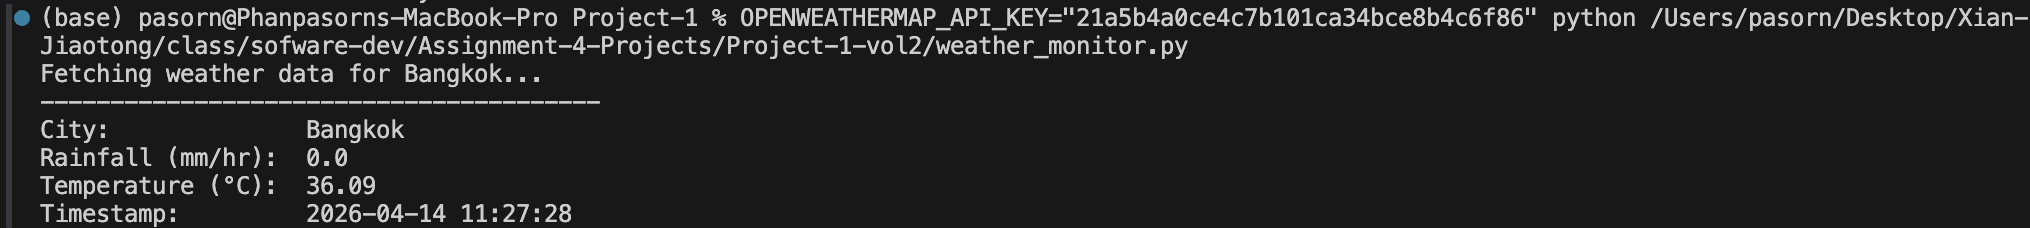
\includegraphics[width=0.9\textwidth]{experiment1-1st-prompt-output.png}
    \caption{Execution output from \texttt{weather\_monitor.py}, displaying retrieved weather parameters}
    \label{fig:API_output}
\end{figure}

% ============================================================
\section{Alert Logic Implementation}
% ============================================================

A threshold-based alert mechanism was developed to classify rainfall intensity into different alert levels. The system evaluates rainfall data and triggers alerts when predefined thresholds are exceeded. In this experiment, a threshold of $\geq 20$ mm/h was used to indicate heavy rainfall conditions.

AI-generated code was used to implement the alert function, which processes incoming weather data and generates alert messages based on the defined criteria. The development workflow, including prompt design, feedback, and execution results, is illustrated in Fig.~\ref{fig:alert_prompt} to Fig.~\ref{fig:Alert_output}.

\subsection{Initial Prompt}

\begin{figure}[H]
    \centering
    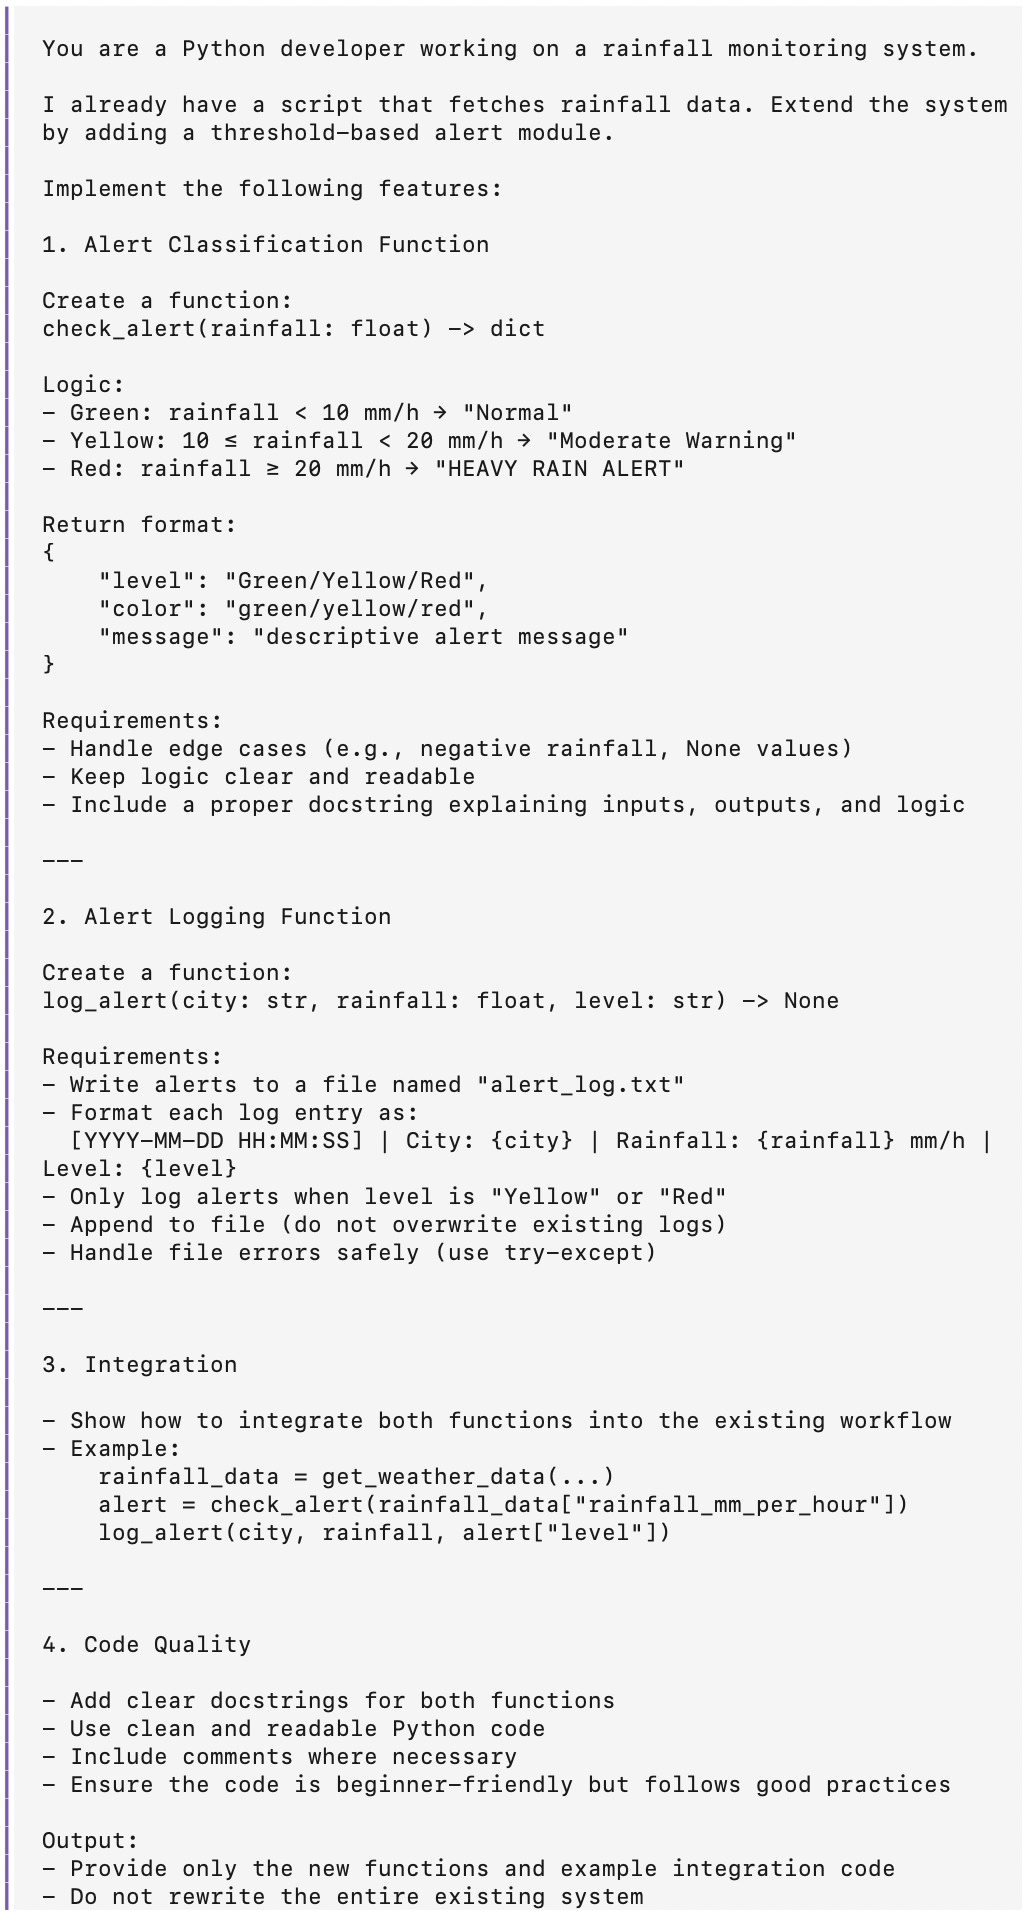
\includegraphics[width=0.9\textwidth]{experiment1-2nd-prompt.png}
    \caption{Initial prompt for \texttt{weather\_alert.py}}
    \label{fig:alert_prompt}
\end{figure}

\subsection{Prompt Feedback}

\begin{figure}[H]
    \centering
    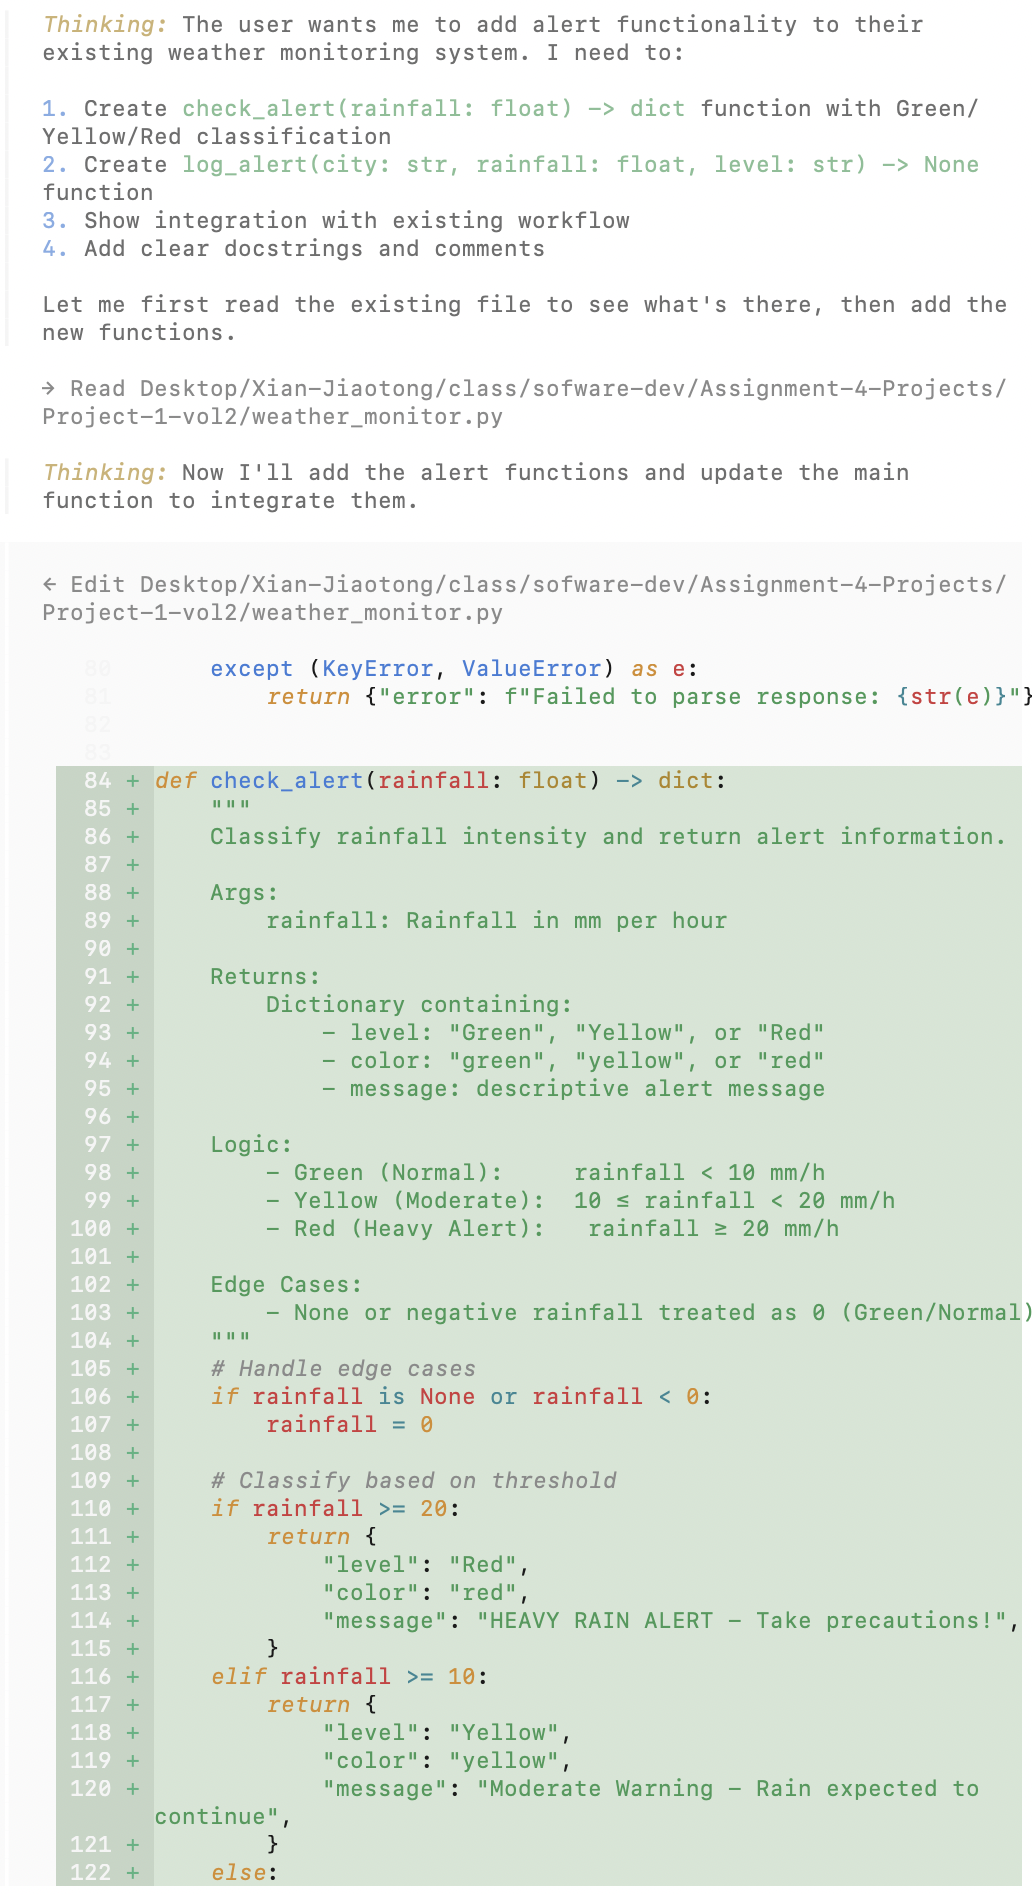
\includegraphics[width=0.9\textwidth]{experiment1-2nd-prompt-feedback1.png}
    \caption{Agent reasoning process for implementing the alert function}
    \label{fig:alert_fb1}
\end{figure}

\begin{figure}[H]
    \centering
    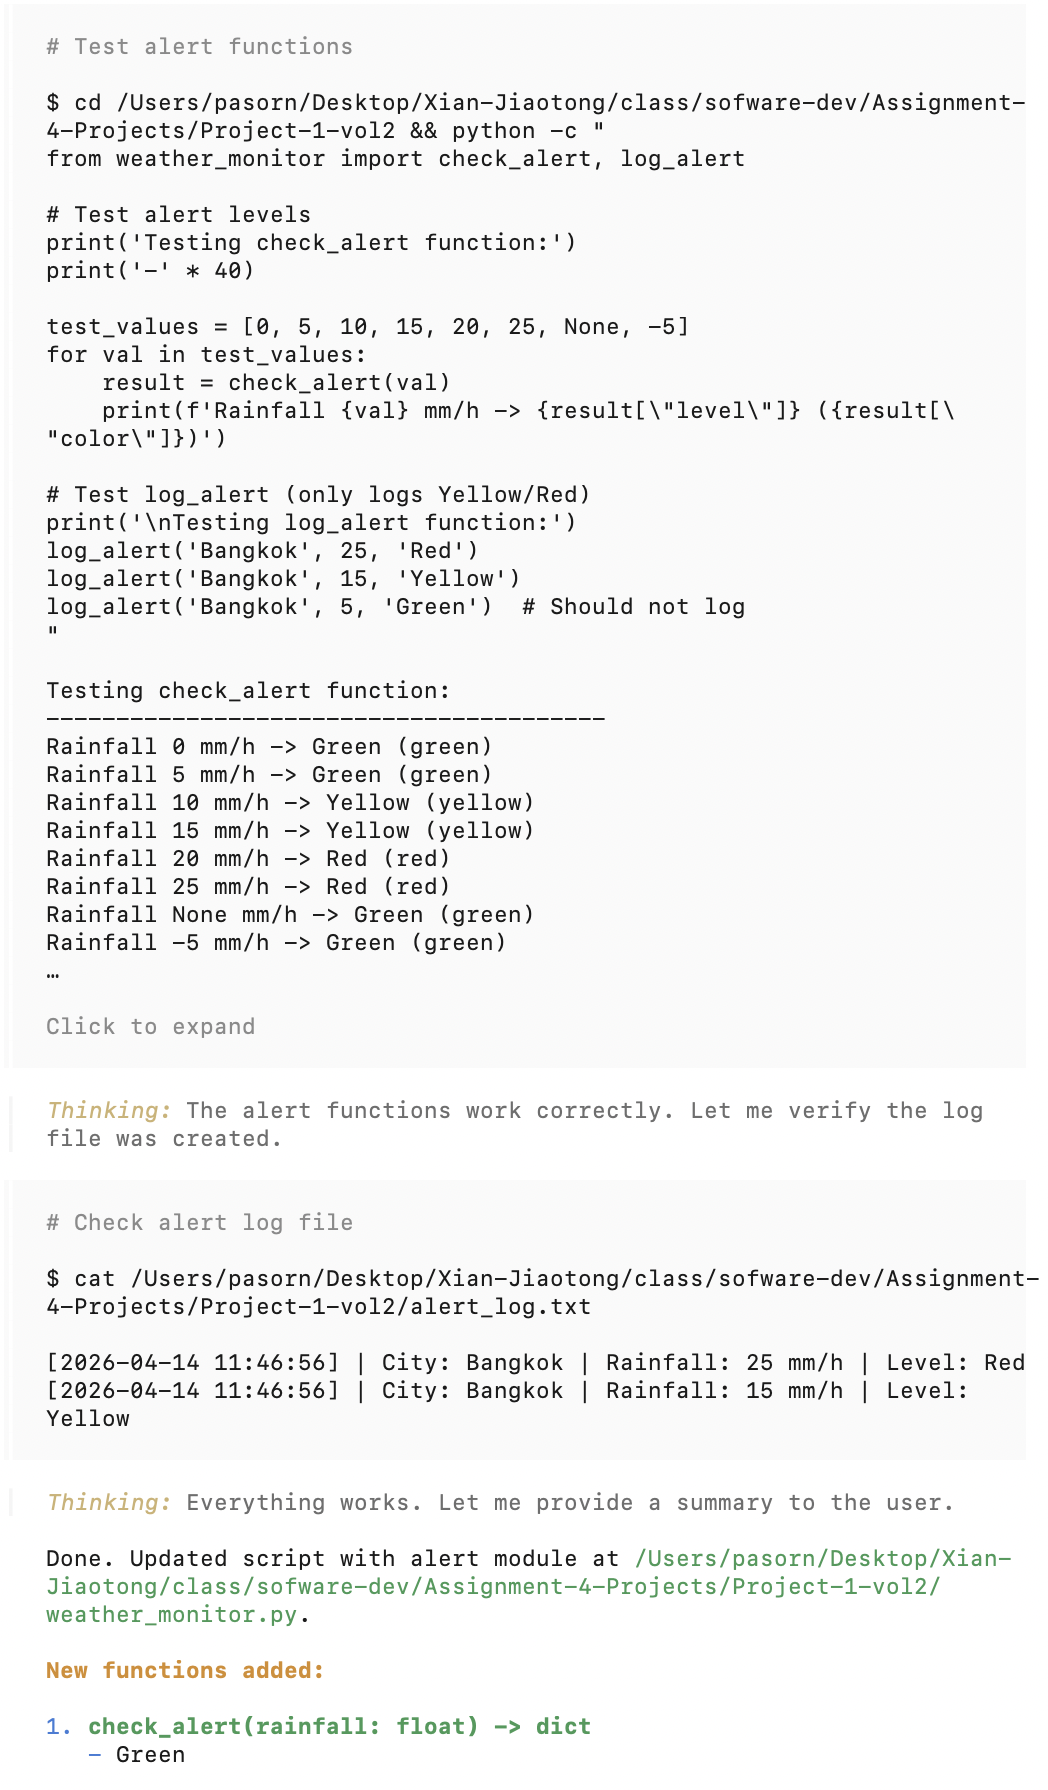
\includegraphics[width=0.9\textwidth]{experiment1-2nd-prompt-feedback3.png}
    \caption{Agent testing and validation of the alert function}
    \label{fig:alert_fb2}
\end{figure}

\subsection{Result}

\begin{figure}[H]
    \centering
    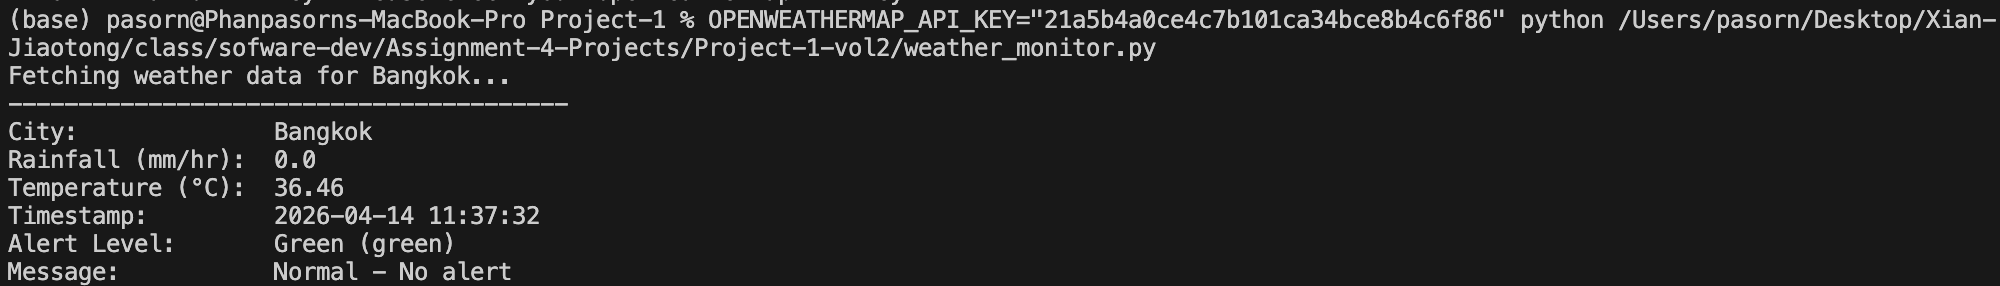
\includegraphics[width=0.9\textwidth]{experiment1-2nd-prompt-output.png}
    \caption{Execution output from \texttt{weather\_alert.py}, showing alert status based on rainfall intensity}
    \label{fig:Alert_output}
\end{figure}

% ============================================================
\section{Dashboard Development}
% ============================================================

A web-based dashboard was developed using Streamlit to visualize real-time weather data and alert status. The interface presents key metrics, color-coded alert indicators and supports automatic updates at regular intervals (5 minutes).

This development stage consists of three iterative prompt refinements. First, Fig.~\ref{fig:dash_prompt1} shows the initial prompt used to create \texttt{weather\_dashboard.py} for real-time monitoring. Second, Fig.~\ref{fig:dash_prompt2} illustrates prompt refinement for improving the user interface. Third, Fig.~\ref{fig:dash_prompt3} focuses on extending functionality to support multi-city monitoring and map-based visualization.

\subsection{Initial Prompt — Dashboard}

\begin{figure}[H]
    \centering
    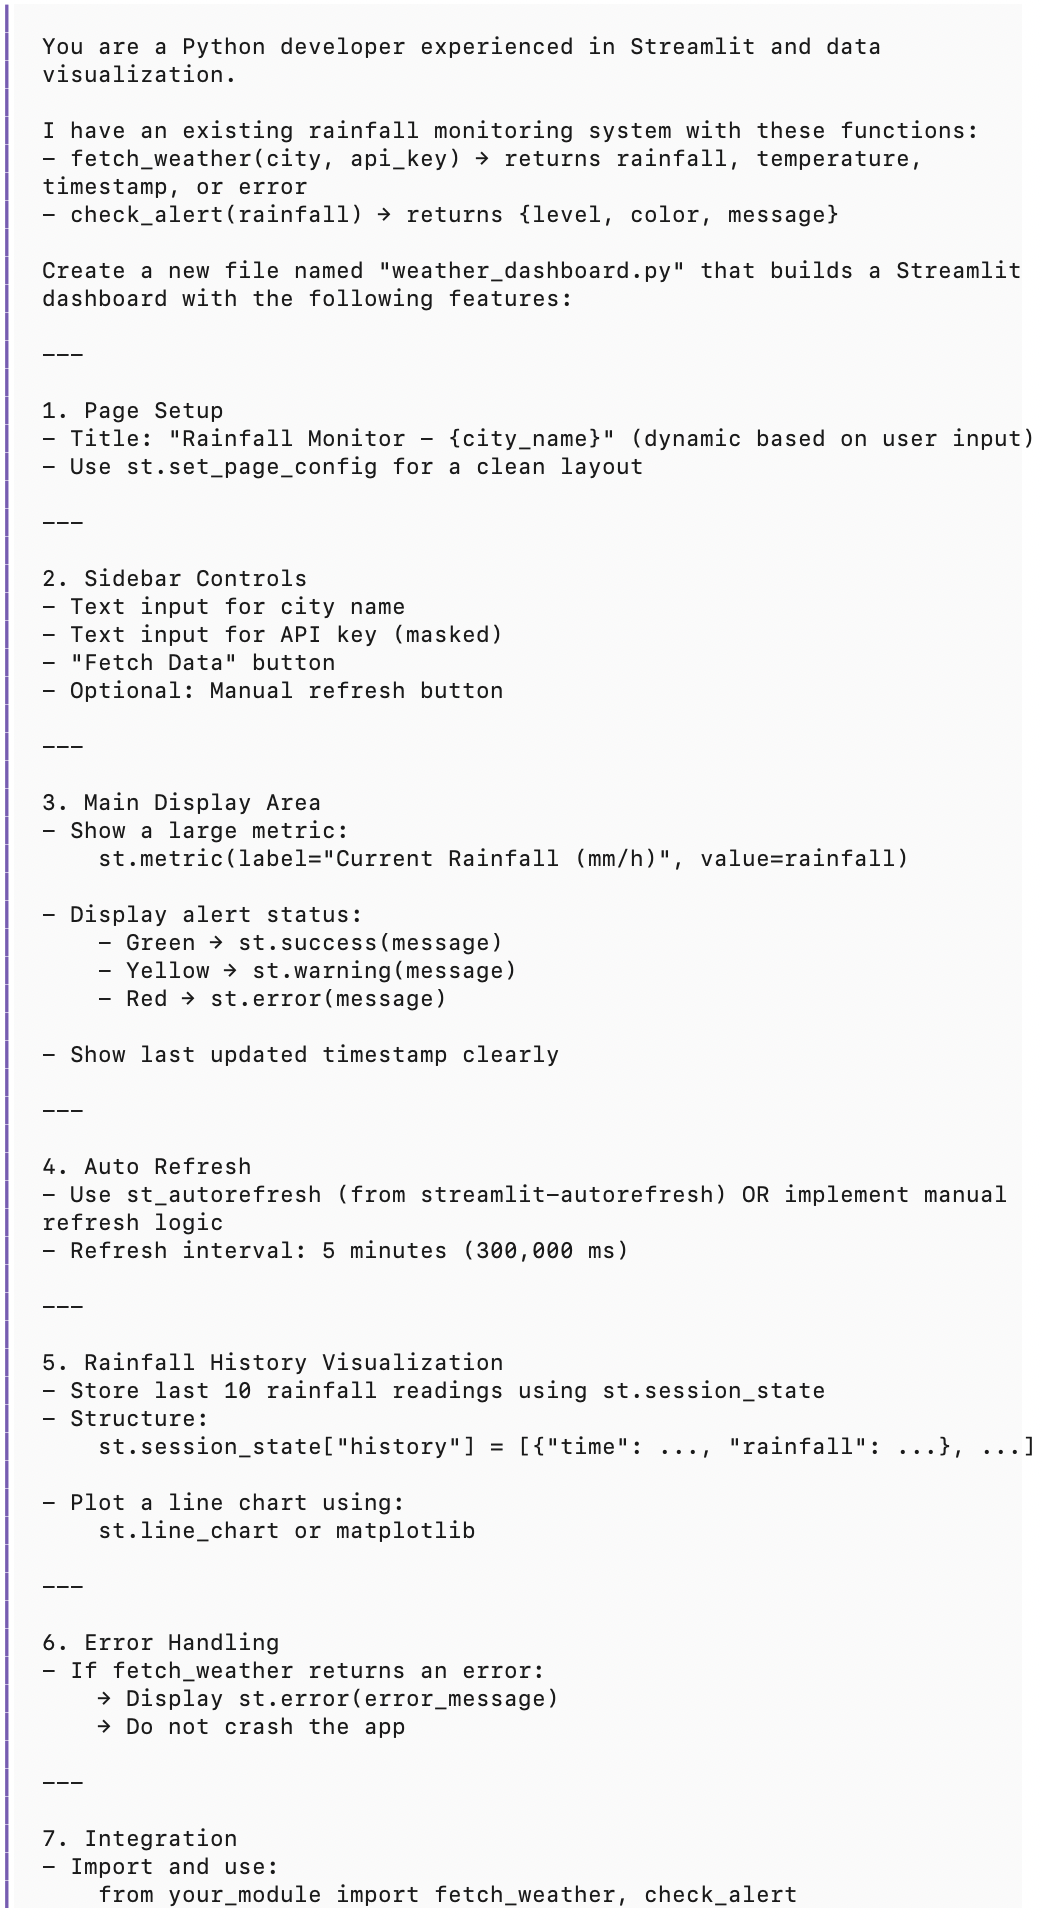
\includegraphics[width=0.9\textwidth]{experiment1-3rd-prompt.png}
    \caption{Initial prompt for \texttt{weather\_dashboard.py} (page 1)}
    \label{fig:dash_prompt1}
\end{figure}

\begin{figure}[H]
    \centering
    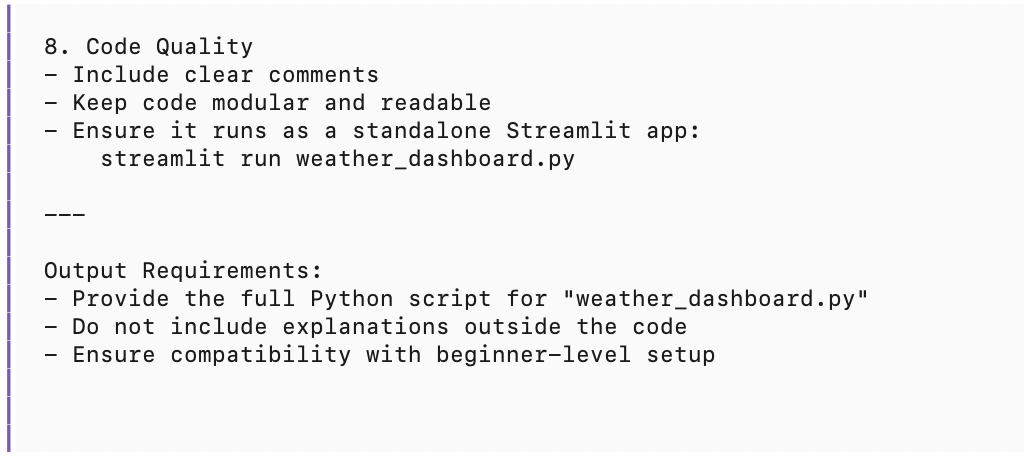
\includegraphics[width=0.9\textwidth]{experiment1-3rd-prompt2.png}
    \caption{Initial prompt for \texttt{weather\_dashboard.py} (page 2)}
    \label{fig:dash_prompt1b}
\end{figure}

\subsection{Prompt Feedback — Dashboard}

\begin{figure}[H]
    \centering
    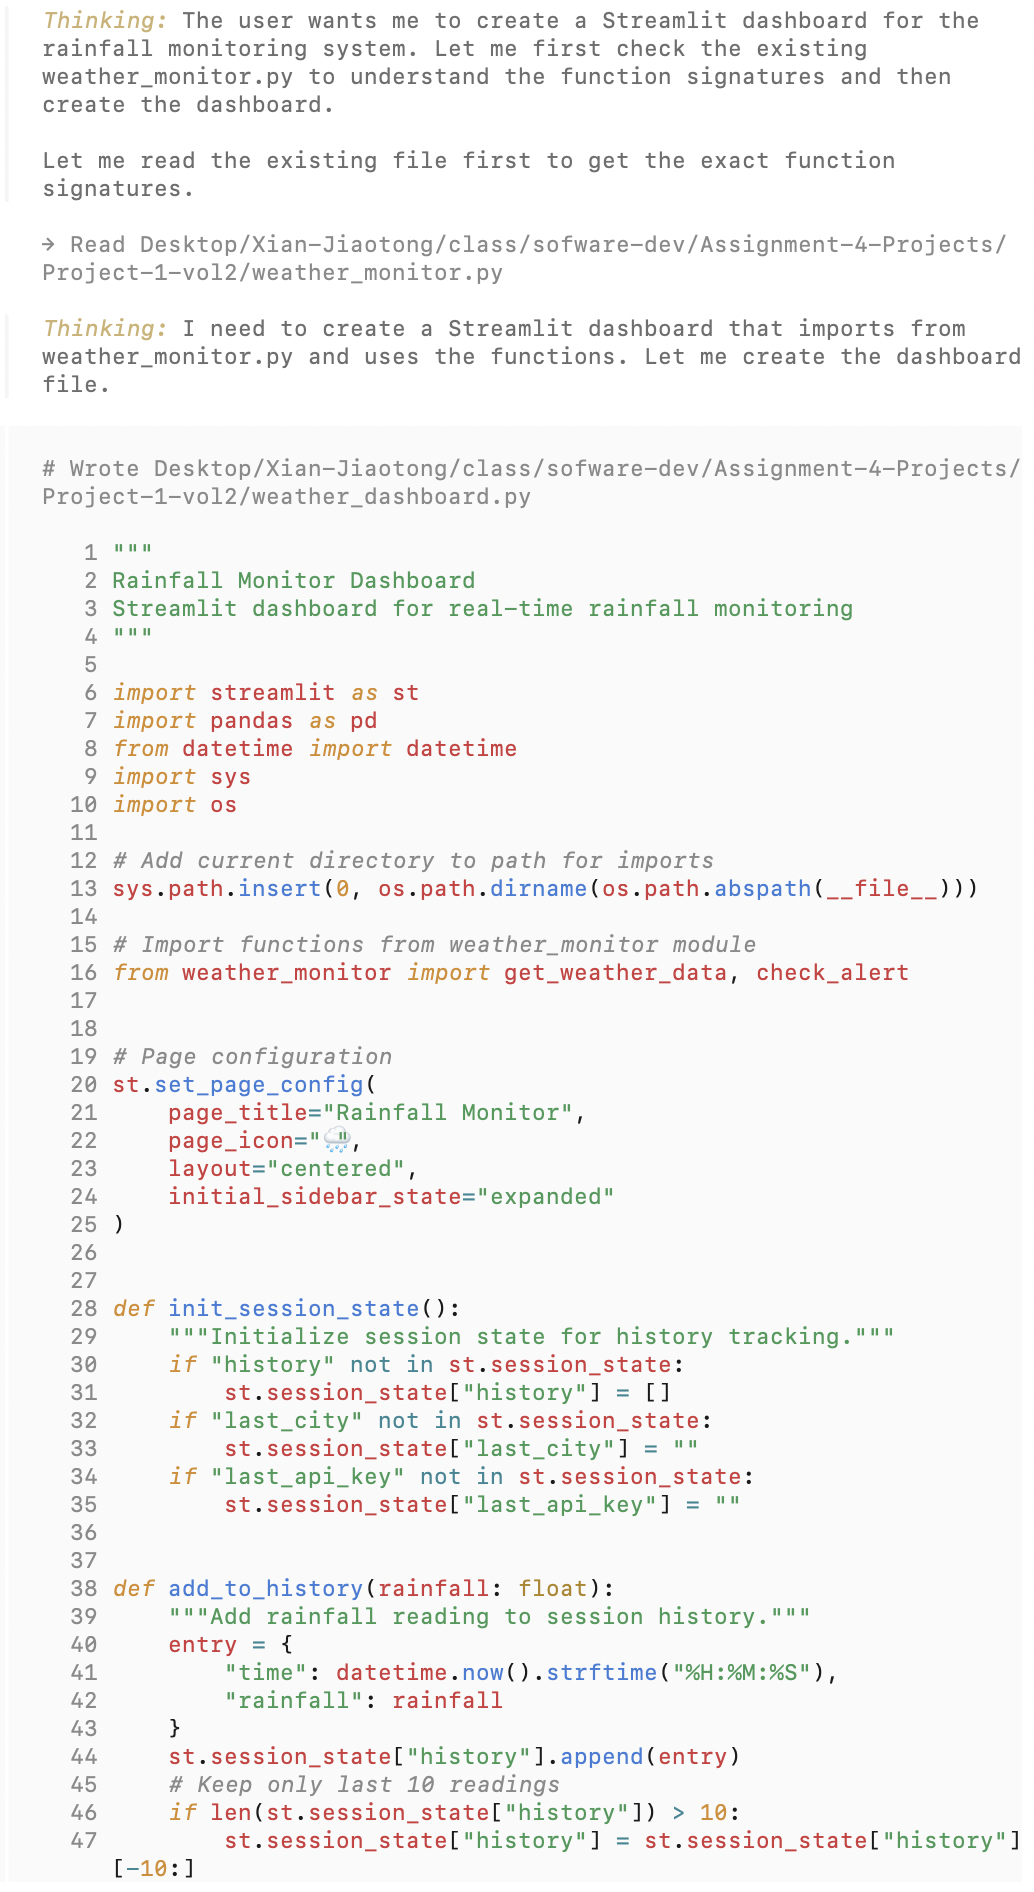
\includegraphics[width=0.9\textwidth]{experiment1-3rd-prompt-feedback1.png}
    \caption{Agent feedback during dashboard development (page 1)}
    \label{fig:dash_fb1}
\end{figure}

\begin{figure}[H]
    \centering
    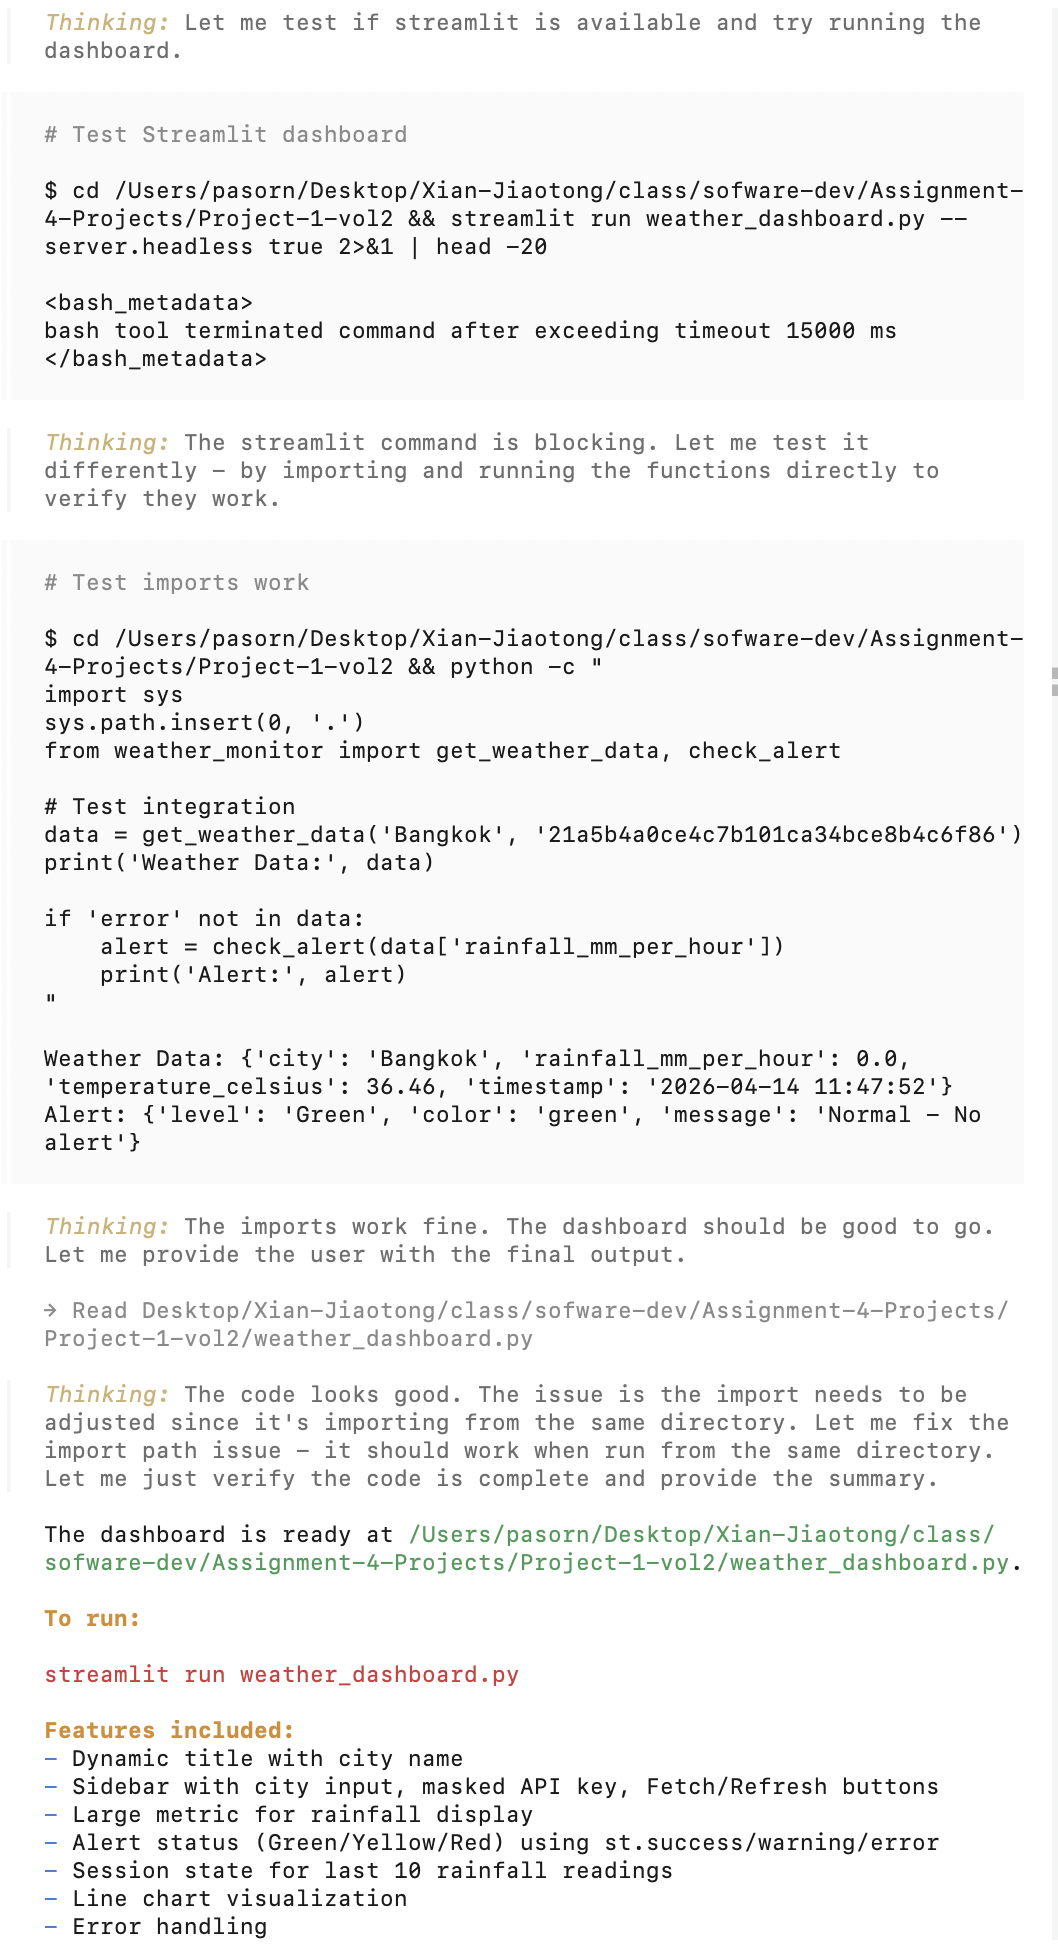
\includegraphics[width=0.9\textwidth]{experiment1-3rd-prompt-feedback2.png}
    \caption{Agent feedback during dashboard development — continued refinement of dashboard logic}
    \label{fig:dash_fb2}
\end{figure}

\subsection{Initial Prompt — UI Improvement}

\begin{figure}[H]
    \centering
    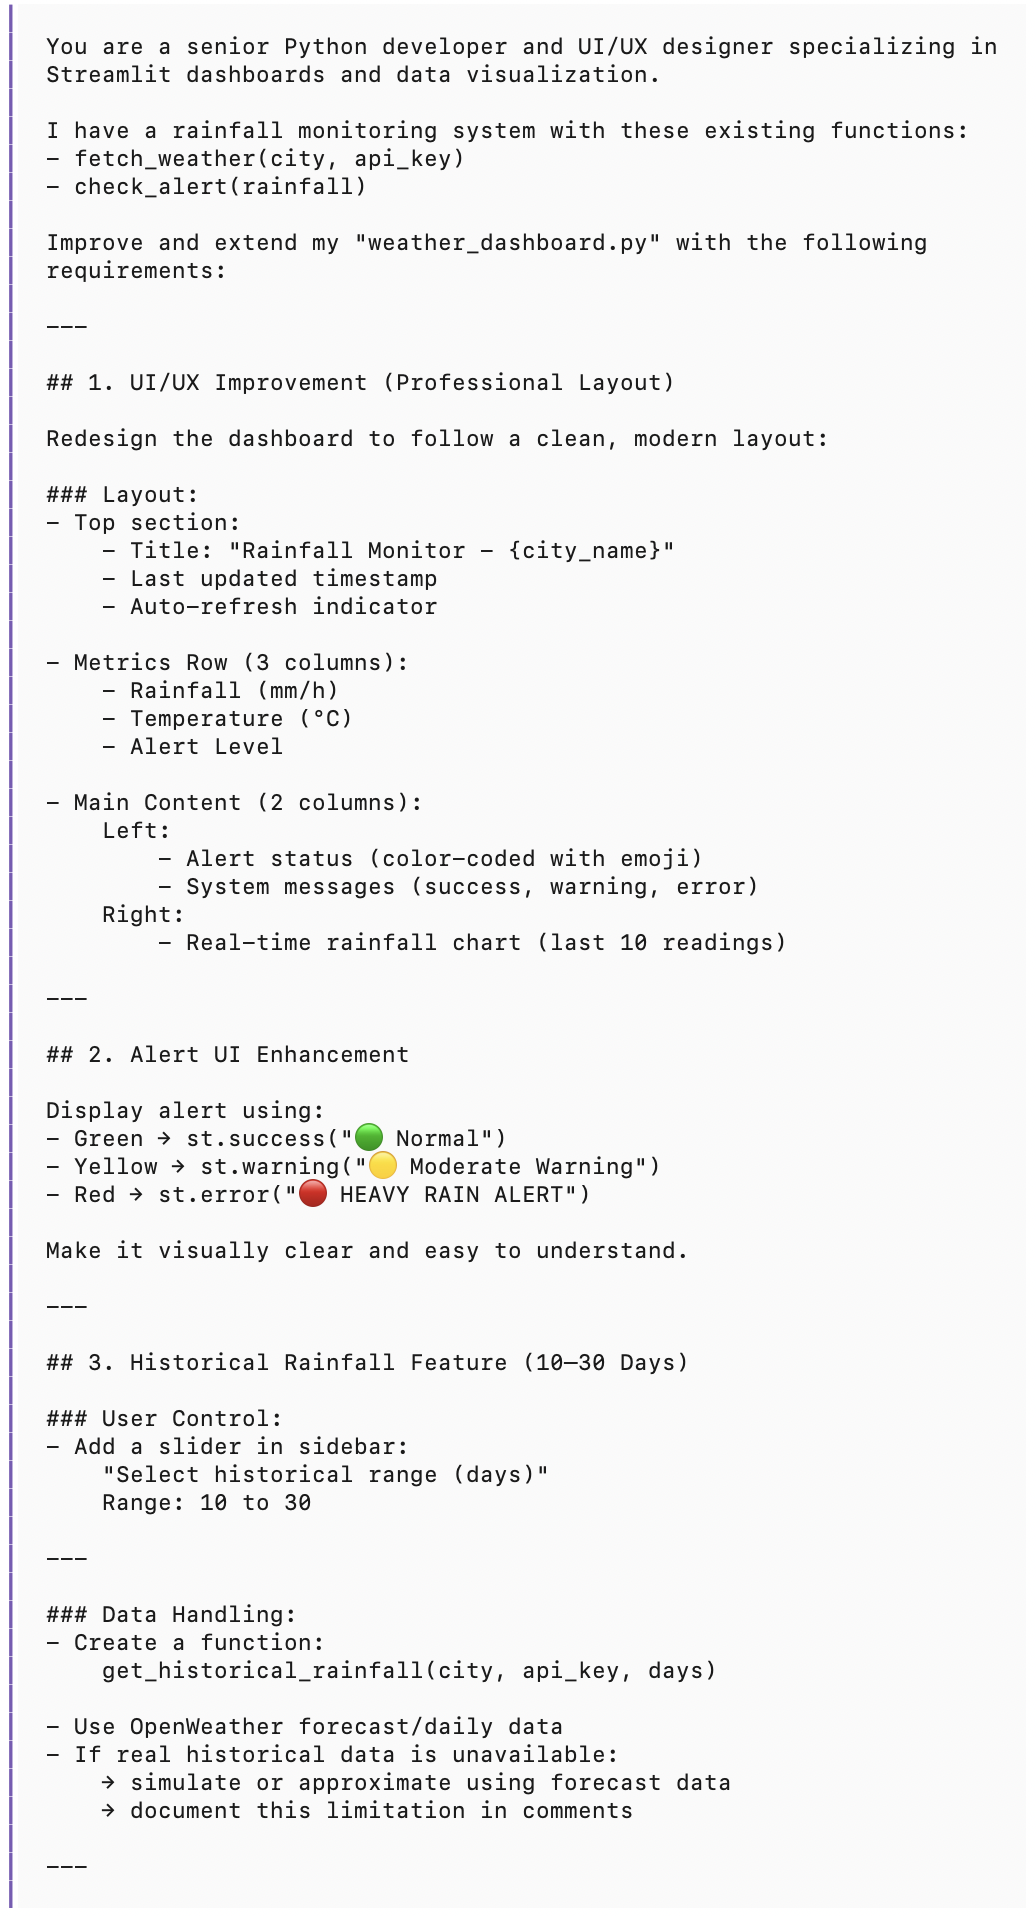
\includegraphics[width=0.9\textwidth]{experiment1-4rd-prompt.png}
    \caption{Prompt for user interface improvement (page 1)}
    \label{fig:dash_prompt2}
\end{figure}

\begin{figure}[H]
    \centering
    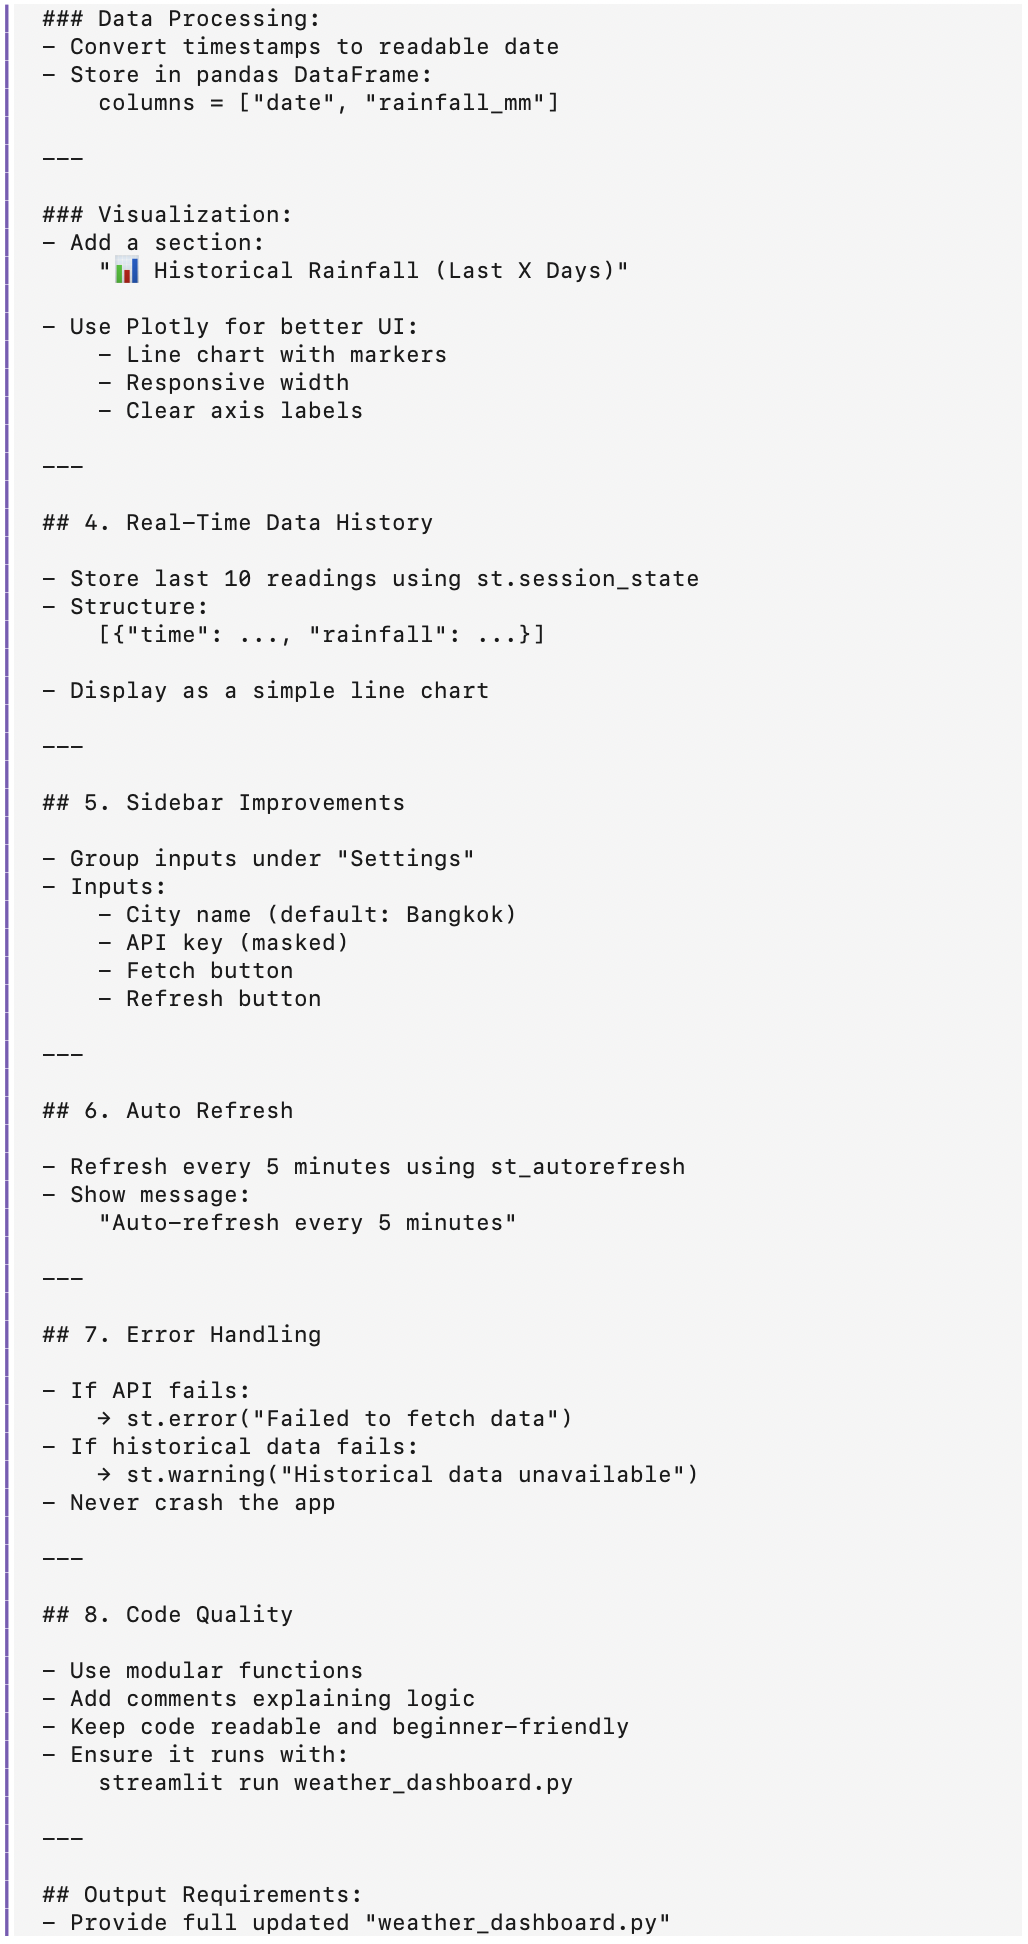
\includegraphics[width=0.9\textwidth]{experiment1-4rd-prompt2.png}
    \caption{Prompt for user interface improvement (page 2)}
    \label{fig:dash_prompt2b}
\end{figure}

\subsection{Prompt Feedback — UI Improvement}

\begin{figure}[H]
    \centering
    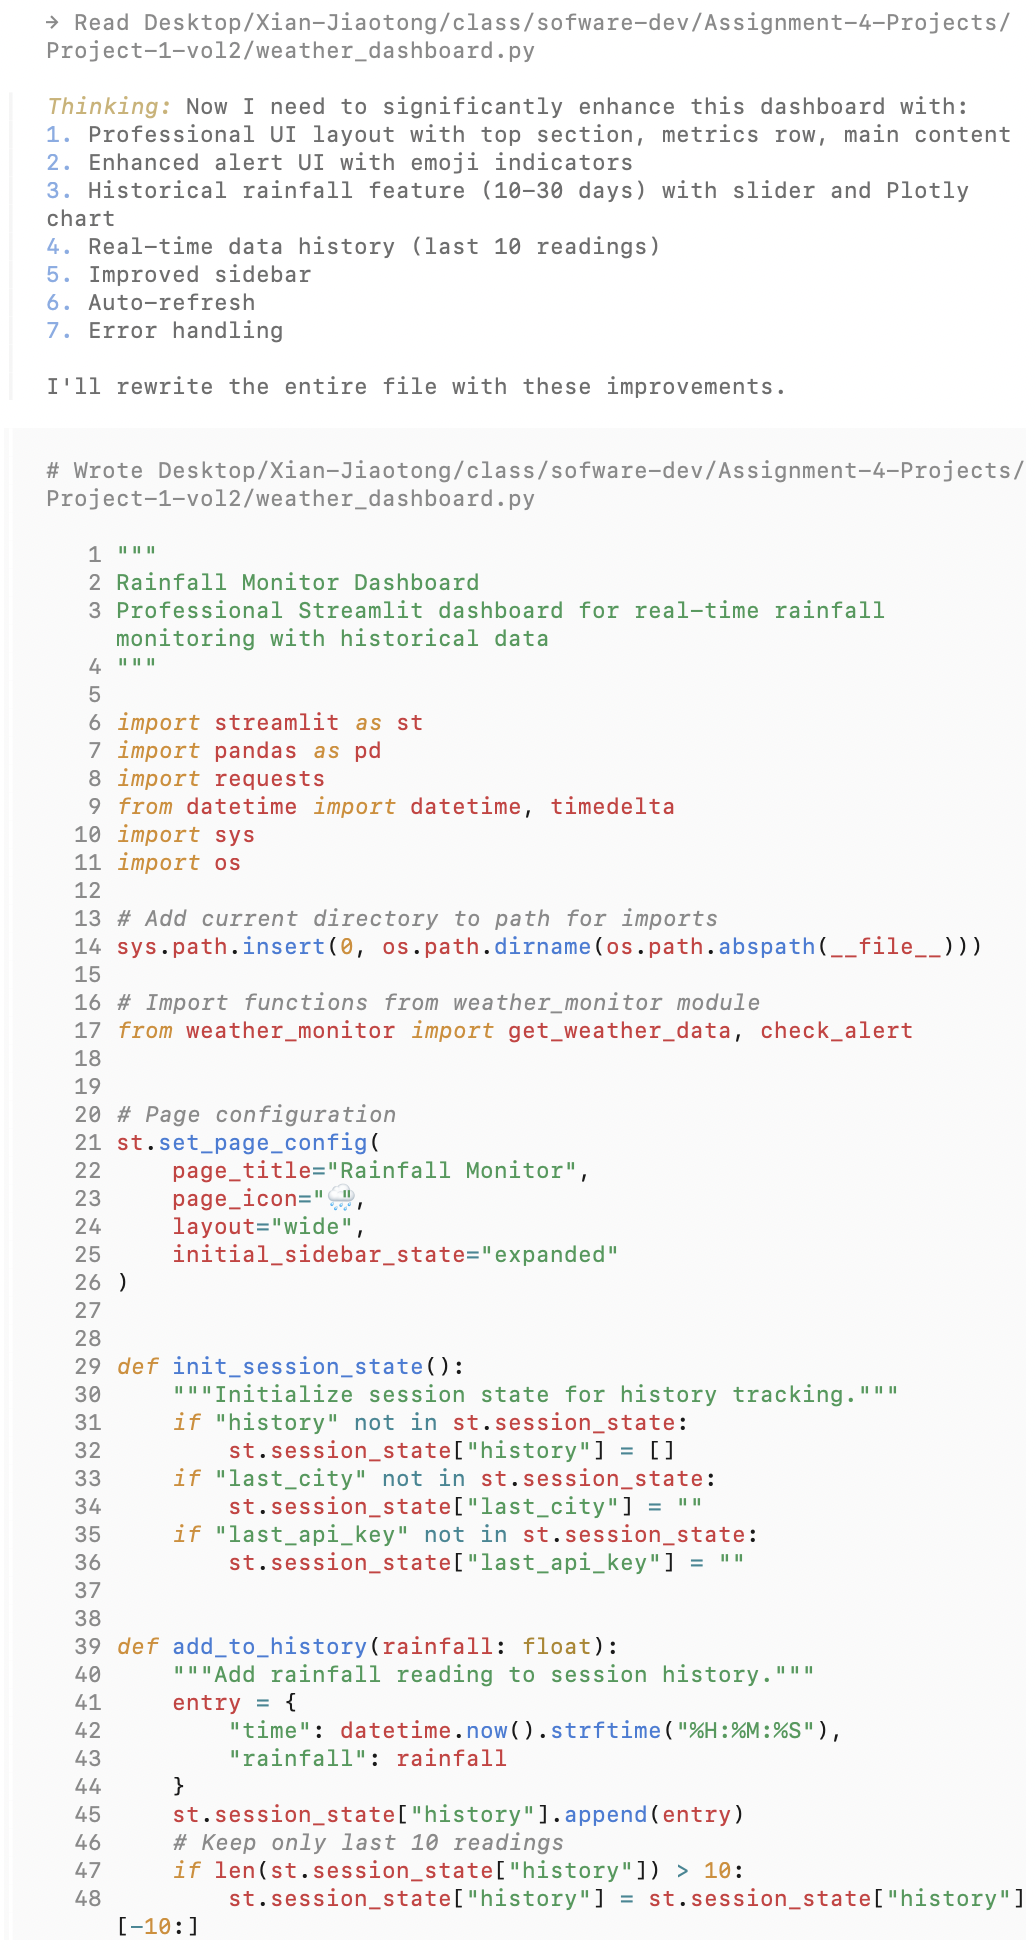
\includegraphics[width=0.9\textwidth]{experiment1-4rd-prompt-feedback1.png}
    \caption{Agent suggestions for UI enhancement}
    \label{fig:dash_fb3}
\end{figure}

\begin{figure}[H]
    \centering
    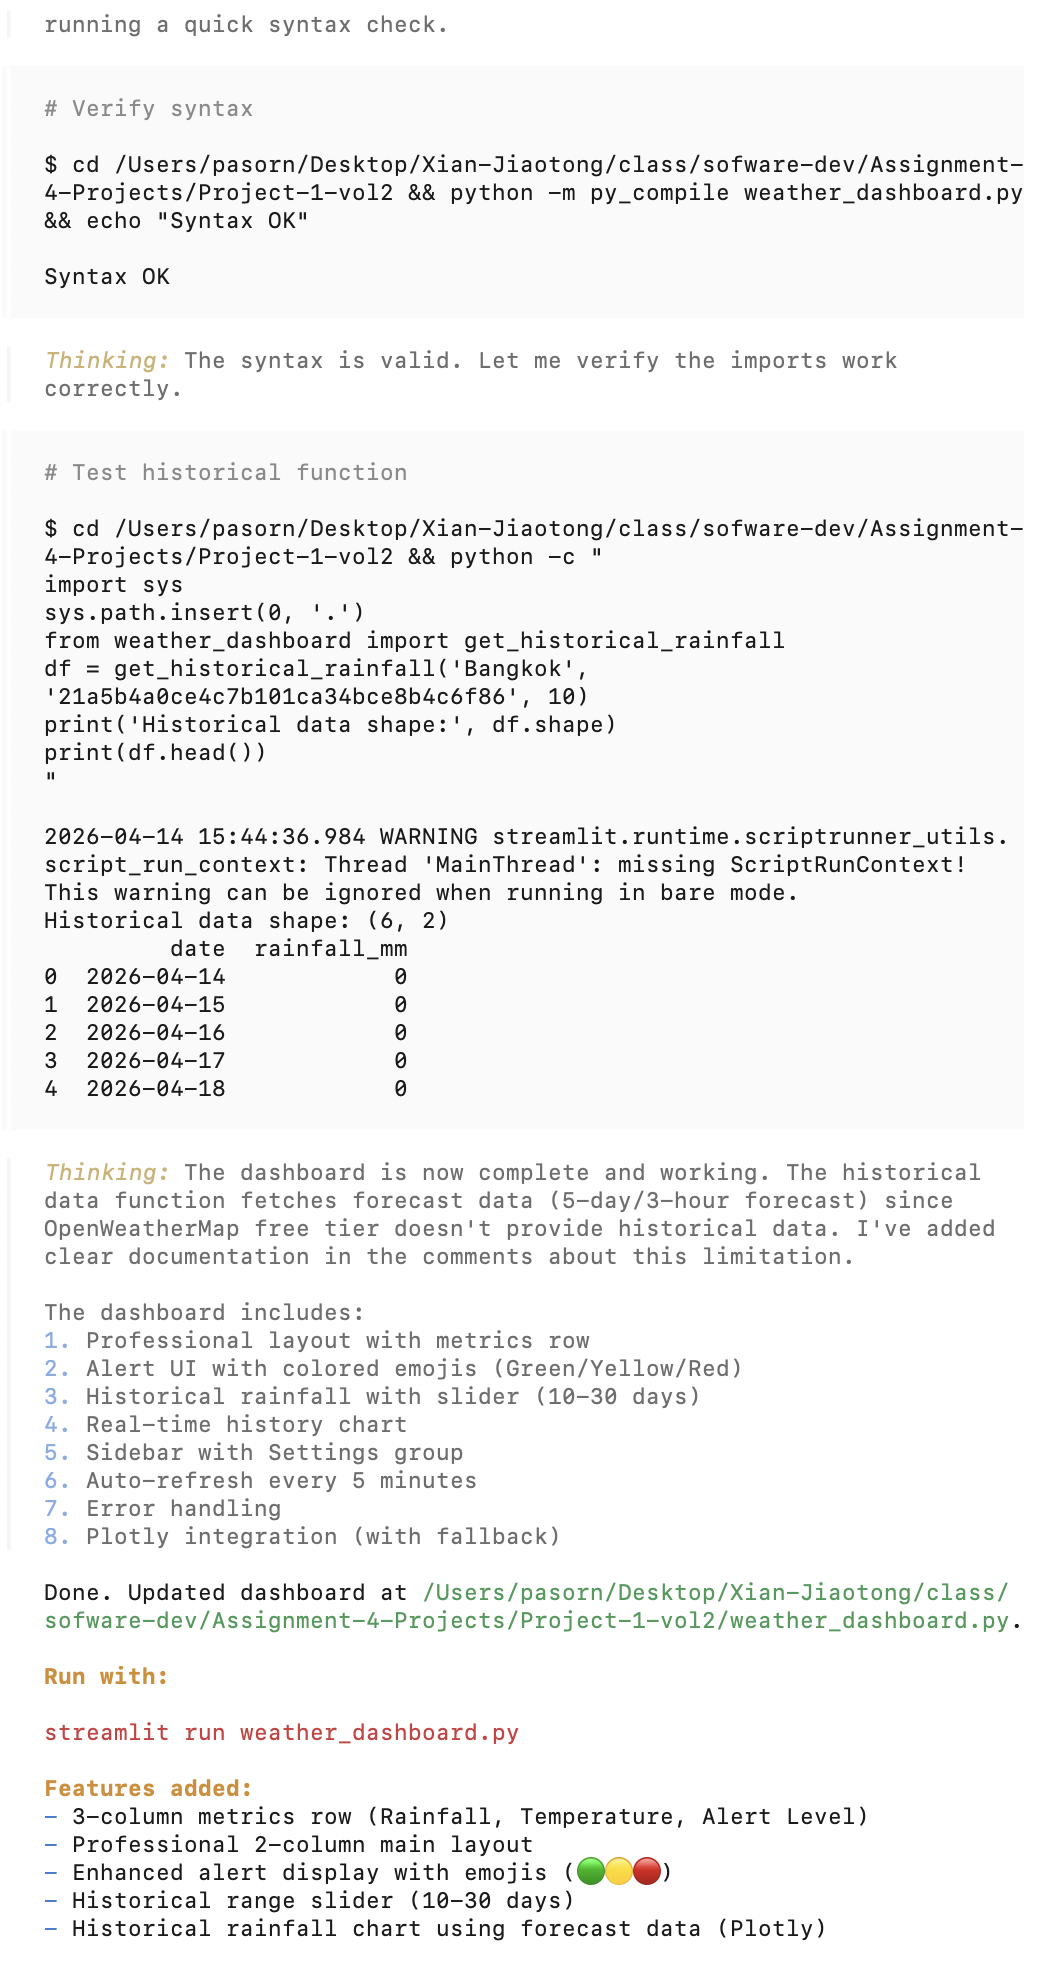
\includegraphics[width=0.9\textwidth]{experiment1-4rd-prompt-feedback2.png}
    \caption{Refined UI implementation feedback}
    \label{fig:dash_fb4}
\end{figure}

\subsection{Initial Prompt — Multi-city \& Map Extension}

\begin{figure}[H]
    \centering
    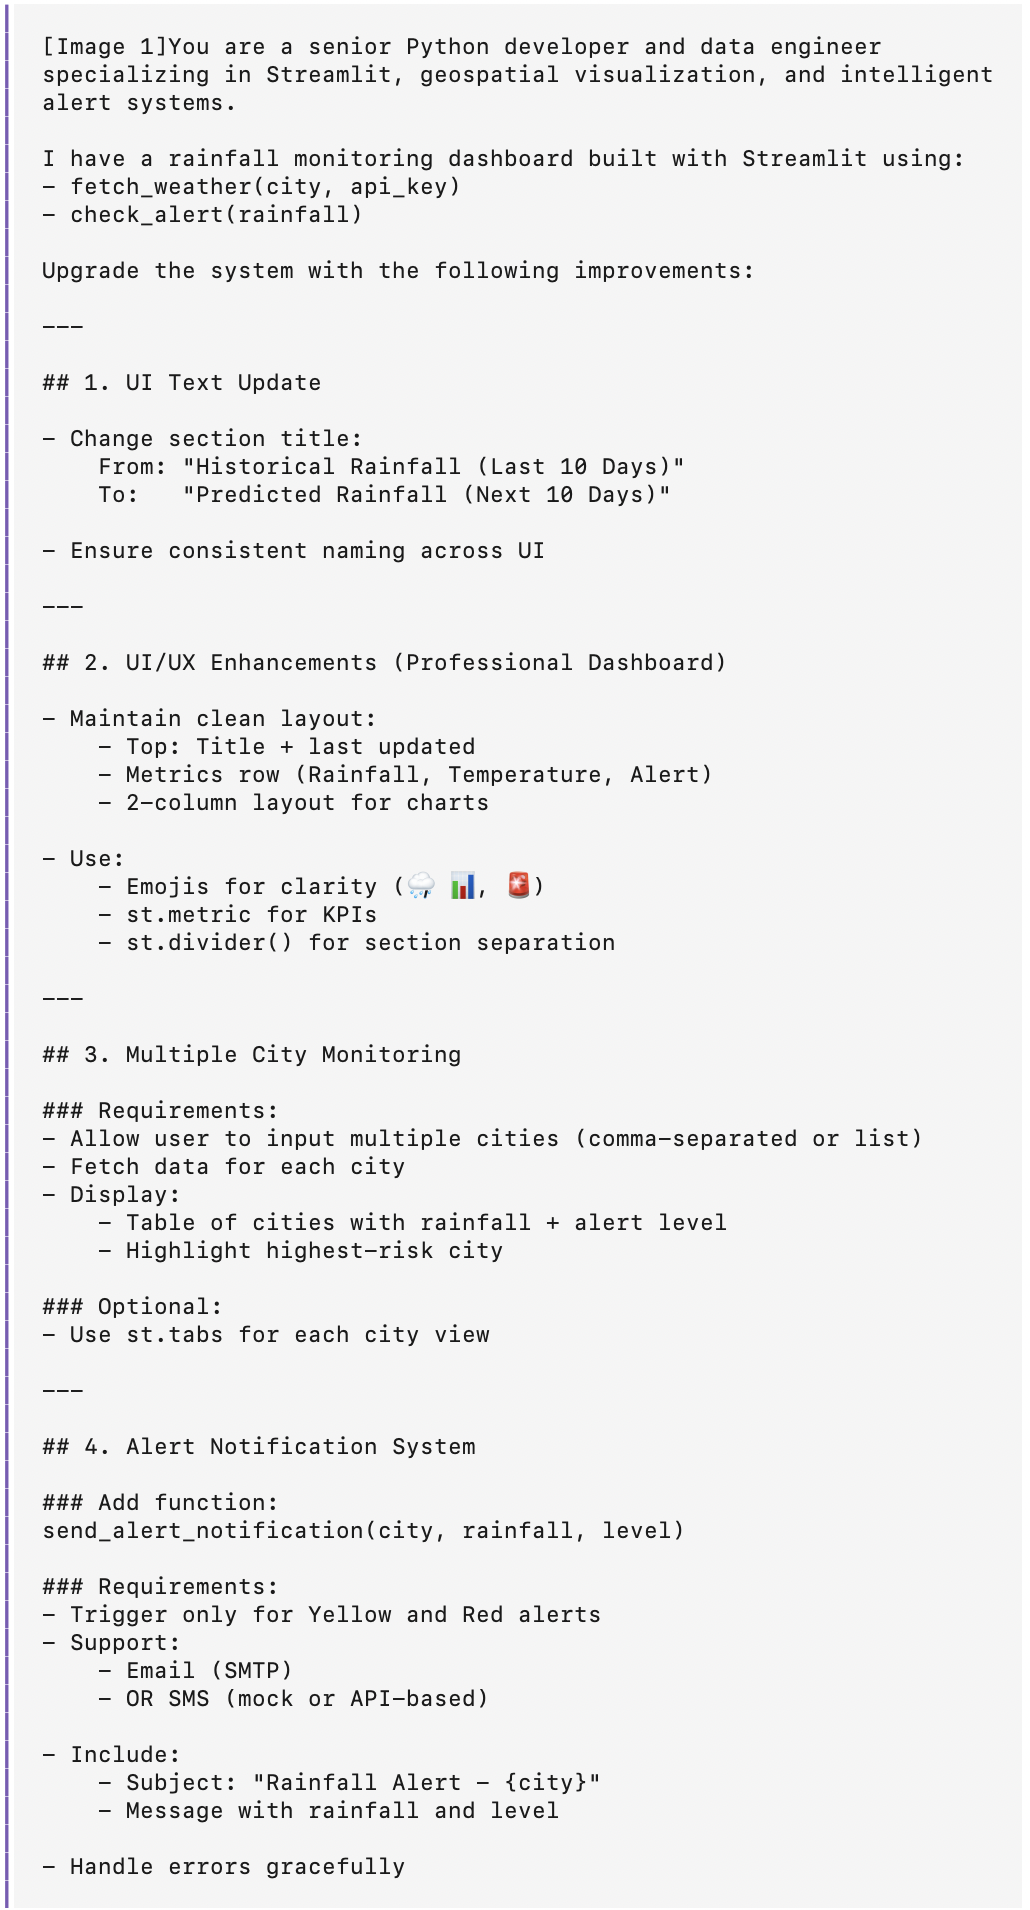
\includegraphics[width=0.9\textwidth]{experiment1-5th-prompt.png}
    \caption{Prompt for multi-city monitoring and map visualization enhancement (page 1)}
    \label{fig:dash_prompt3}
\end{figure}

\begin{figure}[H]
    \centering
    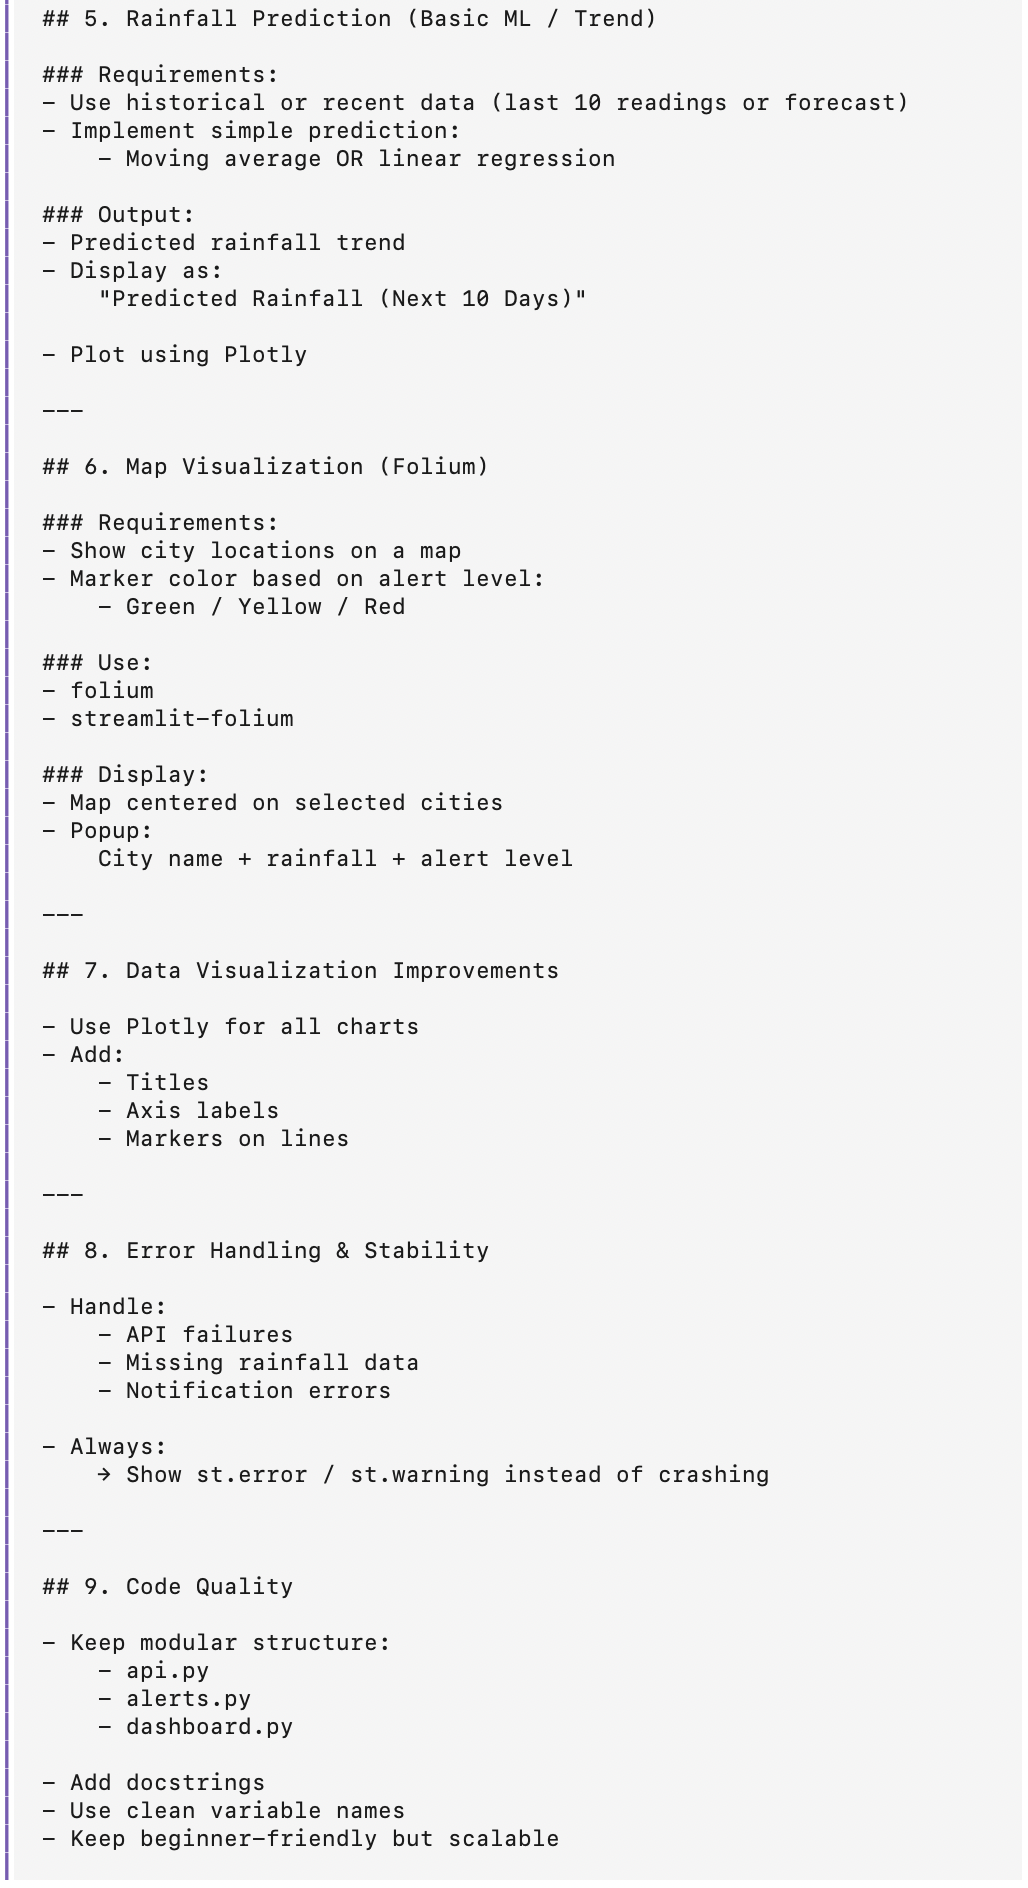
\includegraphics[width=0.9\textwidth]{experiment1-5th-prompt2.png}
    \caption{Prompt for multi-city monitoring and map visualization enhancement (page 2)}
    \label{fig:dash_prompt3b}
\end{figure}

\subsection{Prompt Feedback — Multi-city \& Map Extension}

\begin{figure}[H]
    \centering
    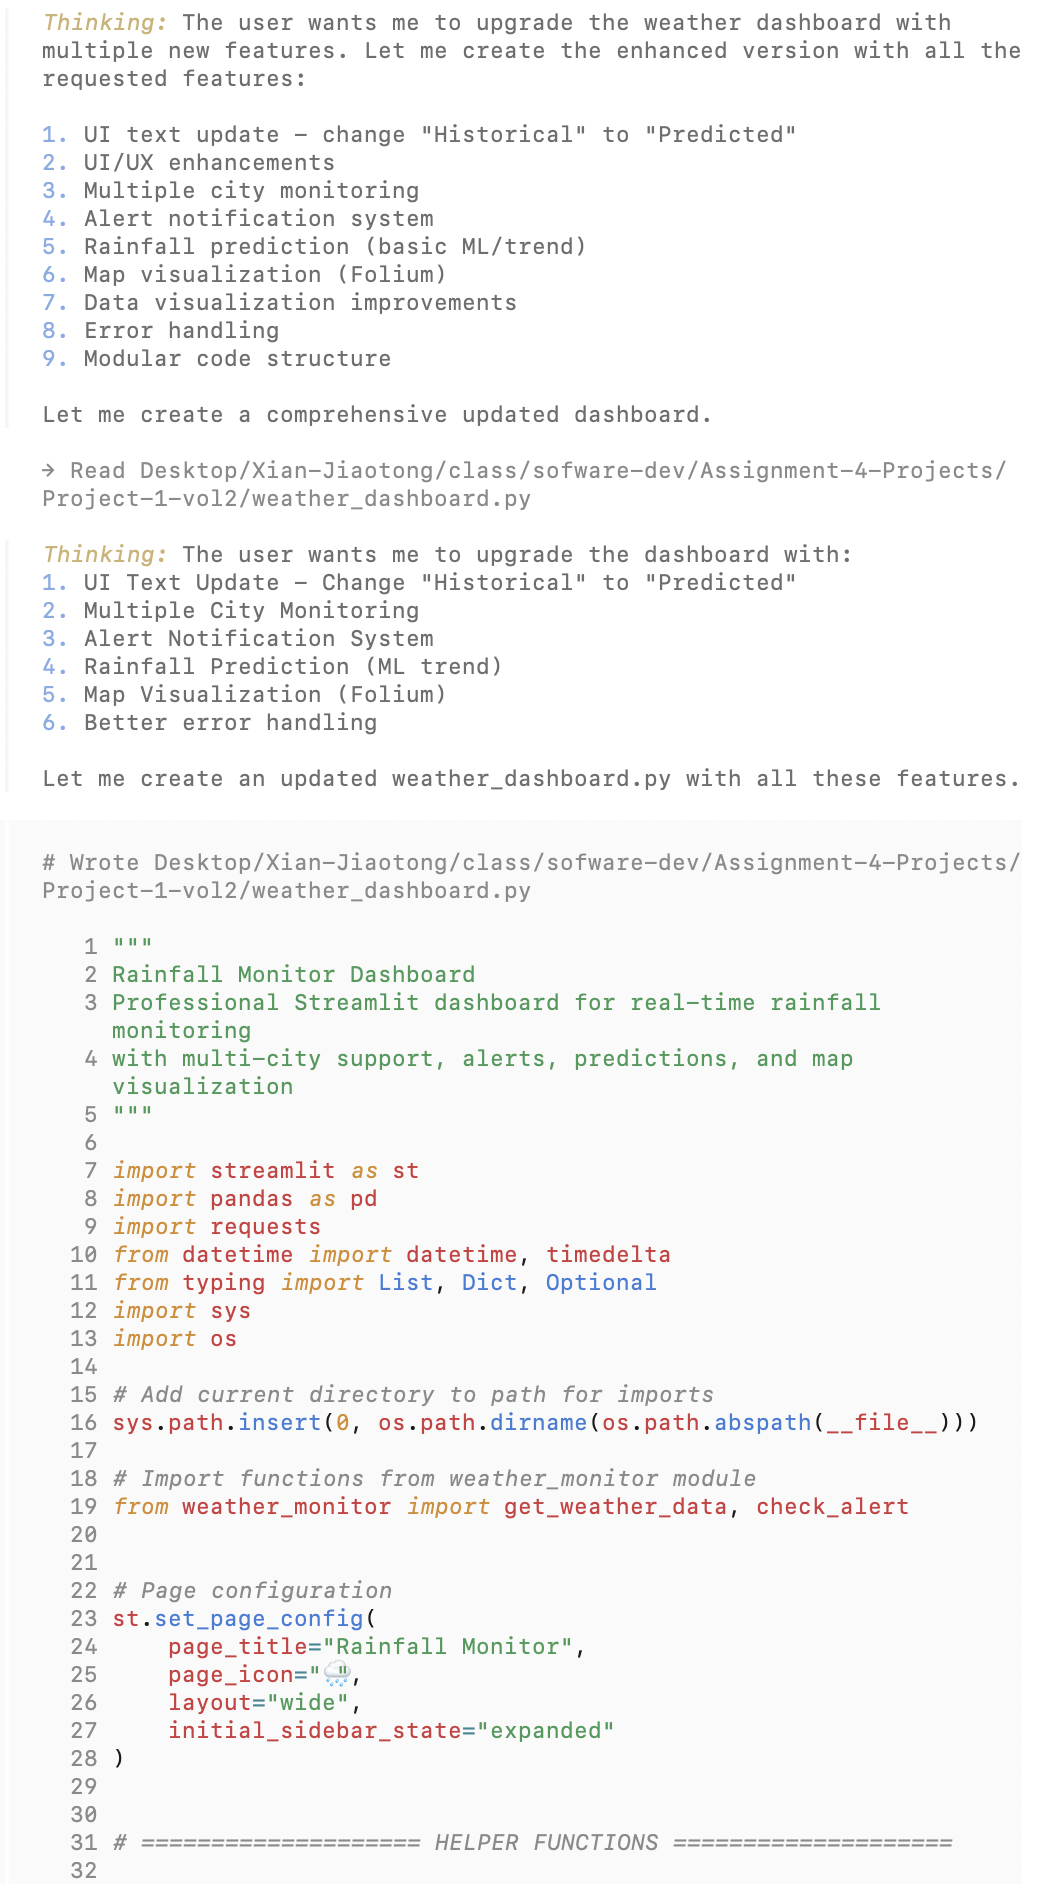
\includegraphics[width=0.9\textwidth]{experiment1-5th-prompt-feedback1.png}
    \caption{Agent feedback — addition of new functional features}
    \label{fig:dash_fb5}
\end{figure}

\begin{figure}[H]
    \centering
    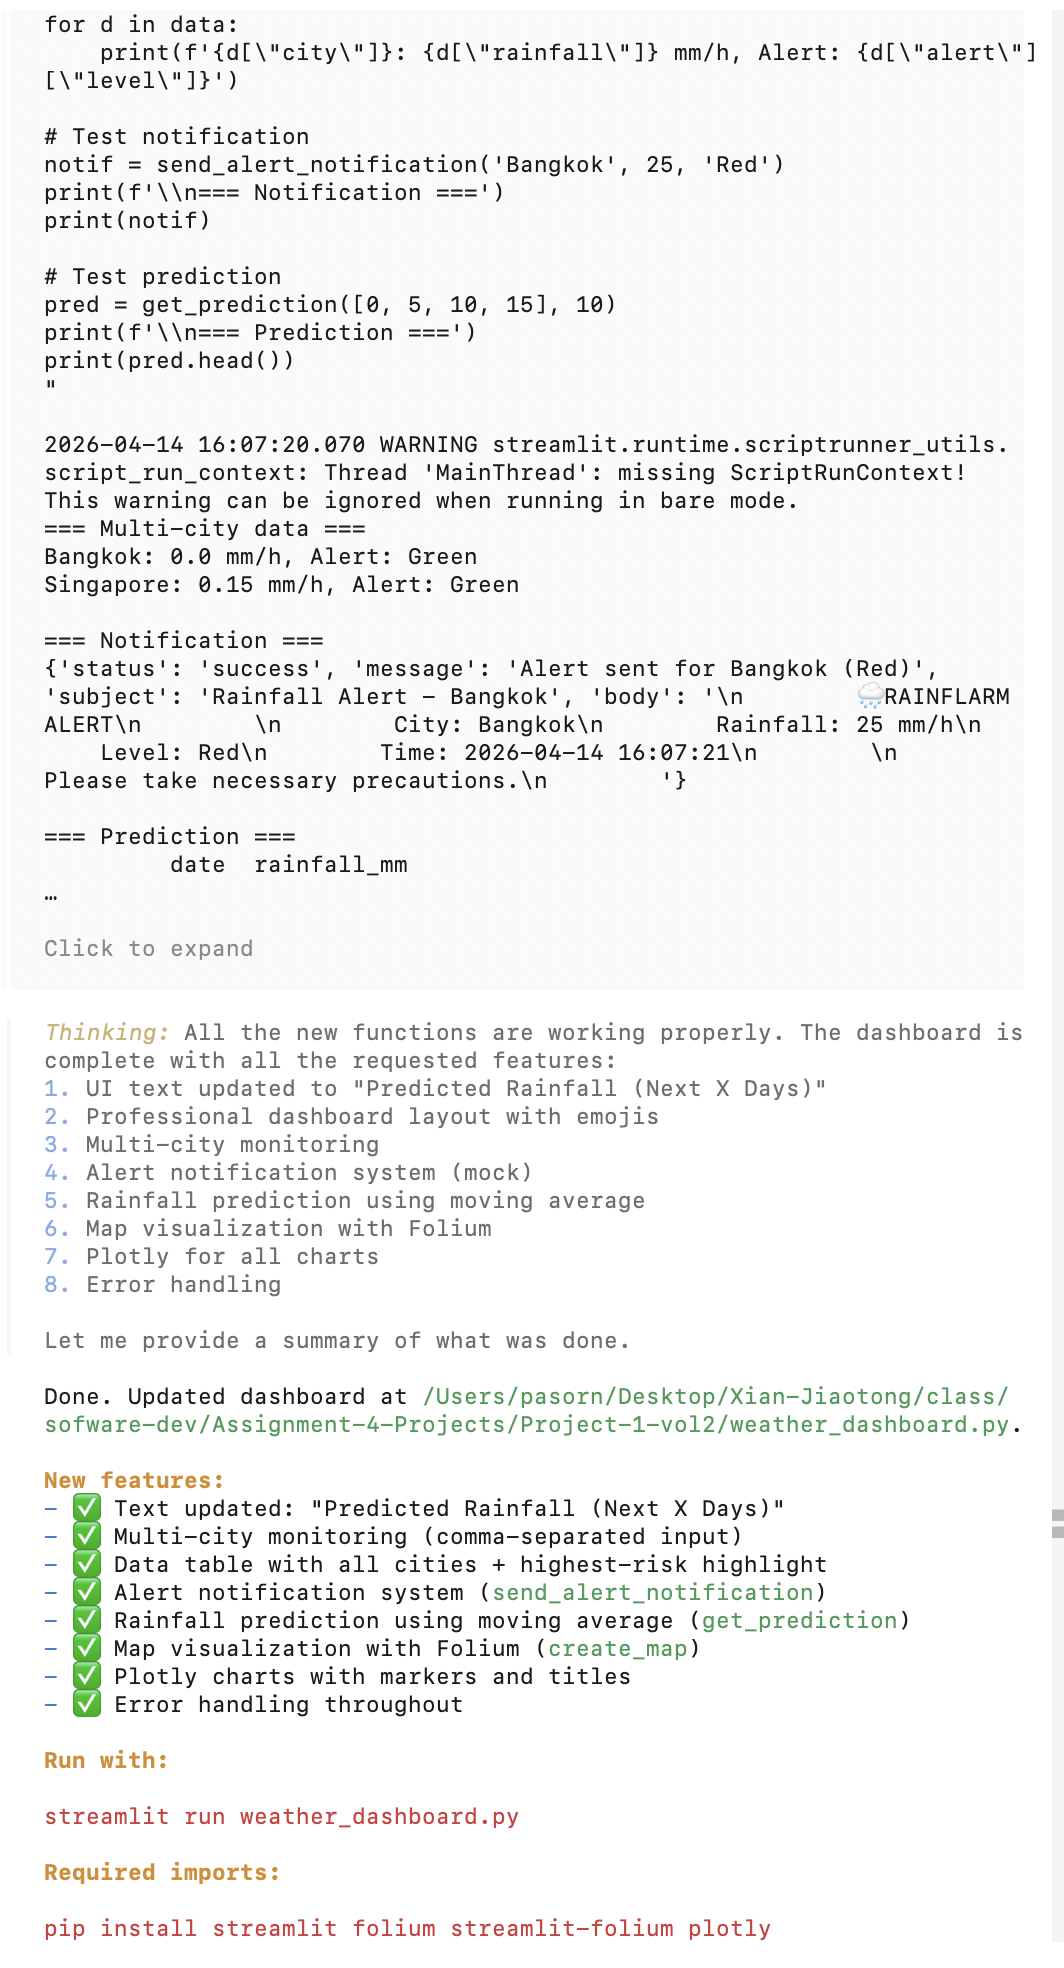
\includegraphics[width=0.9\textwidth]{experiment1-5th-prompt-feedback2.png}
    \caption{Agent feedback — further refinement of system functionality}
    \label{fig:dash_fb6}
\end{figure}

% ============================================================
\section{The Implementation Result}
% ============================================================

The weather monitoring system was successfully implemented using Streamlit. The interface consists of three main components: system configuration for multi-city monitoring, geographical visualization of selected locations, and a 10-day rainfall forecast trend.

\begin{figure}[H]
    \centering
    \includegraphics[width=0.9\textwidth]{experiment1-UI1.png}
    \caption{System configuration and multi-city monitoring overview}
    \label{fig:ui1}
\end{figure}

\begin{figure}[H]
    \centering
    \includegraphics[width=0.9\textwidth]{experiment1-UI2.png}
    \caption{Geographical visualization of selected monitoring locations}
    \label{fig:ui2}
\end{figure}

\begin{figure}[H]
    \centering
    \includegraphics[width=0.9\textwidth]{experiment1-UI3.png}
    \caption{Forecast visualization of rainfall trends}
    \label{fig:ui3}
\end{figure}

% ============================================================
\section{Conclusion}
% ============================================================

The experiment demonstrates that AI-assisted development significantly streamlines the integration of environmental data into actionable software systems. By applying domain-specific rainfall thresholds aligned with heavy rainfall standards, the system provides a reliable tool for real-time urban monitoring.

Furthermore, the integration of API data acquisition, threshold-based alert logic, and interactive dashboard visualization highlights the effectiveness of combining AI-generated code with structured system design.

Future work could extend this framework to support multi-city monitoring, advanced geospatial visualization using libraries such as Folium, and predictive analytics to enhance flood response and decision-making capabilities.

% ============================================================
%  END OF DOCUMENT
% ============================================================
\end{document}
